
\documentclass[12pt,a4paper]{article}
\usepackage[utf8]{inputenc}
\usepackage[T1]{fontenc}
\usepackage[brazil]{babel}
\usepackage{amsmath,amssymb,amsfonts}
\usepackage{graphicx}
\usepackage{booktabs}
\usepackage{hyperref}
\usepackage{minted}
\usepackage{tocloft}
\usepackage{geometry}
\usepackage{csvsimple}
\geometry{margin=2.5cm}
\usepackage{siunitx}
\sisetup{
  round-mode=places,
  round-precision=9,
  table-number-alignment=center,
  detect-all,
  scientific-notation=true
}

\title{PCS5029/PTC5725 -- Aula 06\\\large Introdução aos Métodos Espectrais}
\author{Renan de Luca Avila}
\date{\today}

\begin{document}
\begin{titlepage}
\centering

\includegraphics[width=0.35\textwidth]{EP.jpg}\par\vspace{1cm}
{\scshape\LARGE Escola Politécnica da Universidade de São Paulo\par}
\vspace{1.5cm}
{\huge\bfseries Aula 06 -- Métodos Espectrais\par}
\vspace{0.5cm}
{\Large Resolução da tarefa\par}
\vfill
{\large Renan de Luca Avila\par}
{\large \today\par}
\end{titlepage}

\tableofcontents
\newpage

\section{Resumo}
Este relatório implementa, em Python, os exercícios apresentados nos slides da Aula 06 (Prof.\ Osvaldo Guimarães), e discute as soluções. O documento contém códigos completos, figuras e tabelas, além de apêndices com setup e fontes.

\section{Resoluções}
Cada resolução é apresentada com planejamento, resultados, conclusão e implementação. Os códigos completos estão no Apêndice~\ref{ap:codigos}.

% \subsection{Exercício X}

% \subsubsection{Enunciado}
% % Descreva o enunciado aqui com os detalhes matemáticos

% \subsubsection{Planejamento e fundamentos teóricos}
% % Descreva o plano para resolver o problema e cite os fundamentos teóricos que sustentam o plano, incluindo fórmulas e equações justificando o caminho escolhido

% \subsubsection{Etapas de implementação e funções principais}
% % Coloque citações de trechos do código aqui e explique o que cada uma delas faz relacionando com os fundamentos teóricos (use minted referenciando códigos da pasta /code)

% \subsubsection{Resultados e discussão}
% % Coloque aqui figuras (da pasta /figures) e tabelas (da pasta /tables) que mostrem os resultados obtidos como saída do código e interprete os resultados

% \subsubsection{Conclusão}
% % Resuma o que fizemos para resolver e conclua com avaliações dos resultado

\newpage

\subsection{Exercício 1}

\subsubsection{Enunciado}
Resolver numericamente o problema de contorno não linear
\begin{equation}
u''(x) = e^{u(x)}, \qquad x \in [-1,1],
\end{equation}
com condições de contorno de Dirichlet
\begin{equation}
u(-1) = u(1) = 1.
\end{equation}
Deseja-se:
\begin{enumerate}
    \item Obter a solução numérica $u(x)$ via método de Newton combinado com discretização espectral de Chebyshev;
    \item Calcular e plotar o resíduo $R(x)=u''(x)-e^{u(x)}$;
    \item Comparar o resultado com a solução analítica da forma
    \begin{equation}
        u(x) = \ln\!\left(\frac{a^2}{1+\cos(a x)}\right),
    \end{equation}
    onde o parâmetro $a$ é determinado da condição $u(1)=1$, ou seja:
    \begin{equation}
        a^2 = e\,[1+\cos(a)].
    \end{equation}
\end{enumerate}

\subsubsection{Planejamento e fundamentos teóricos}
O problema é não linear devido à presença do termo $e^{u(x)}$. Para discretizar espacialmente, aplicamos o \textbf{método espectral de Chebyshev} com pontos de colocação de Gauss--Lobatto:
\begin{equation}
x_j = \cos\!\left(\frac{j\pi}{N}\right), \qquad j = 0,\ldots,N.
\end{equation}

A matriz de diferenciação $D$ é construída a partir da fórmula clássica (Trefethen, \emph{Spectral Methods in MATLAB}):
\begin{equation}
D_{ij} = 
\begin{cases}
\dfrac{c_i}{c_j}\dfrac{1}{x_i-x_j}, & i \neq j,\\[1em]
-\displaystyle\sum_{k\neq i} D_{ik}, & i=j,
\end{cases}
\quad 
c_0=c_N=2,\; c_j=1 \text{ para } 1\le j\le N-1.
\end{equation}
Com $D^2 = D\,D$ obtém-se a aproximação espectral da segunda derivada $u'' \approx D^2 u$.

Assim, o sistema residual é
\begin{equation}
R(u) = D^2 u - e^{u} = 0,
\end{equation}
cuja forma linearizada em Newton é
\begin{equation}
J\,\delta u = -R(u), \qquad J = D^2 - \mathrm{diag}(e^{u}),
\end{equation}
atualizando $u \leftarrow u + \delta u$ apenas nos pontos internos (as fronteiras são conhecidas).

\subsubsection{Etapas de implementação e funções principais}
O código foi implementado em \texttt{Python} (arquivo \texttt{/code/tarefa1\_bvp.py}) utilizando o \texttt{NumPy} e o \texttt{Matplotlib}.  
O trecho abaixo mostra a construção das matrizes espectrais de Chebyshev:

\begin{minted}[fontsize=\small,breaklines,frame=lines]{python}
def cheb_D_matrices(N):
    k = np.arange(0, N+1)
    x = np.cos(np.pi * k / N)[::-1]
    X = np.tile(x, (N+1,1))
    dX = X - X.T
    c = np.ones(N+1); c[0]=2; c[-1]=2
    c = c * ((-1)**np.arange(N+1))
    C = np.tile(c, (N+1,1))
    D = (C.T / C) / (dX + np.eye(N+1))
    D = D - np.diag(np.sum(D, axis=1))
    D2 = D @ D
    return x, D, D2
\end{minted}

O laço de Newton resolve o sistema linear $J\,\delta u=-R$ até convergência:

\begin{minted}[fontsize=\small,breaklines,frame=lines]{python}
for it in range(maxit):
    R = D2 @ u - np.exp(u)
    r = R[1:-1]
    J = D2[np.ix_(idx_int, idx_int)] - np.diag(np.exp(u[idx_int]))
    du_int = solve(J, -r)
    u[1:-1] += du_int
\end{minted}

Por fim, o parâmetro $a^*$ da solução analítica é ajustado pela condição de contorno $a^2=e(1+\cos a)$ via método de Newton:

\begin{minted}[fontsize=\small,breaklines,frame=lines]{python}
def find_a_newton(a0=2.0, tol=1e-14):
    a = a0
    for _ in range(100):
        fa = a*a - np.e*(1+np.cos(a))
        dfa = 2*a + np.e*np.sin(a)
        a -= fa / dfa
        if abs(fa) < tol:
            break
    return a
\end{minted}

\subsubsection{Resultados e discussão}
As Figuras~\ref{fig:u_solucao}, \ref{fig:residuo} e \ref{fig:newton} apresentam os resultados obtidos.

\begin{figure}[H]
    \centering
    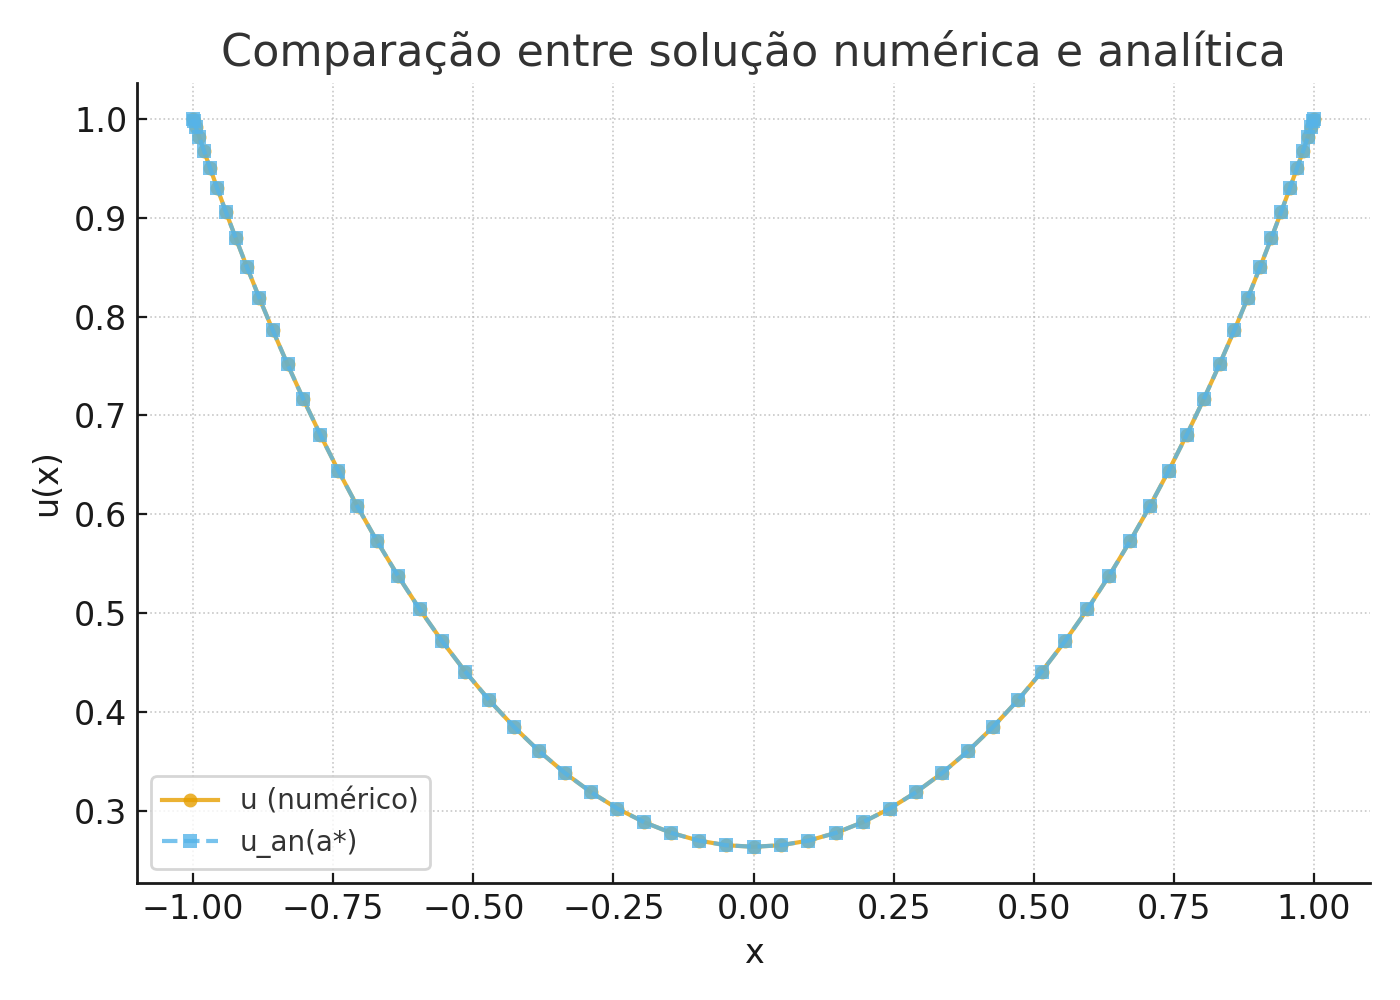
\includegraphics[width=0.75\textwidth]{figures/u_solution_highlighted.png}
    \caption{Soluções numérica (círculos) e analítica (quadrados) para $u''=e^u$.}
    \label{fig:u_solucao}
\end{figure}

\begin{figure}[H]
    \centering
    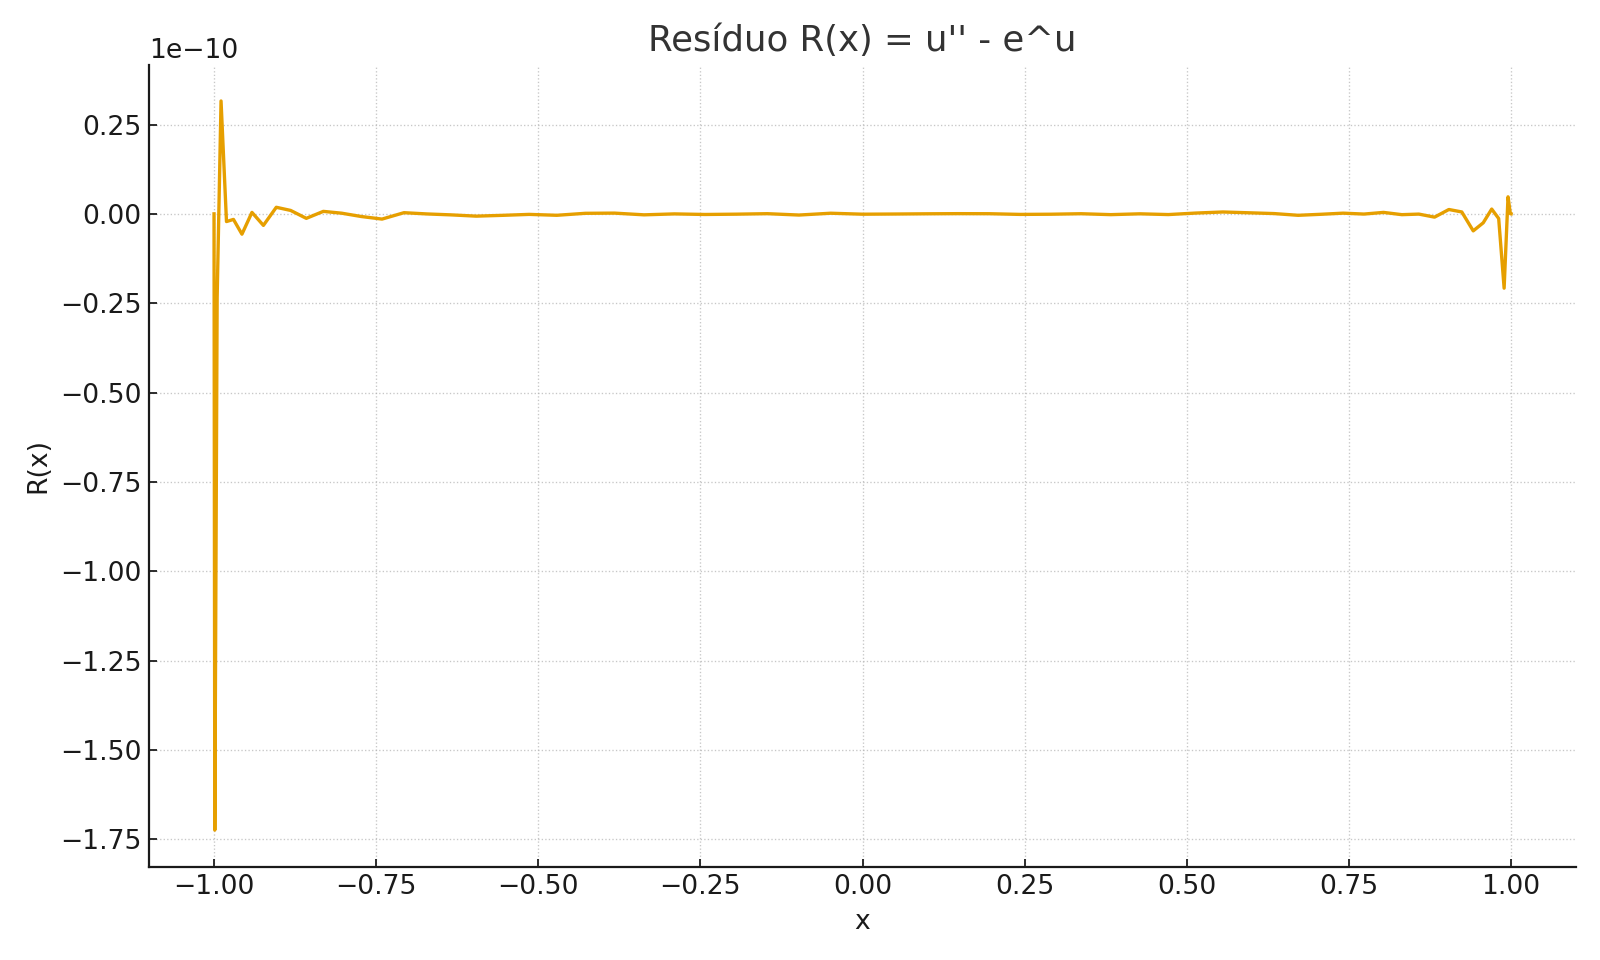
\includegraphics[width=0.65\textwidth]{figures/residual.png}
    \caption{Resíduo espectral $R(x)=u''-e^u$ nos nós de Chebyshev.}
    \label{fig:residuo}
\end{figure}

\begin{figure}[H]
    \centering
    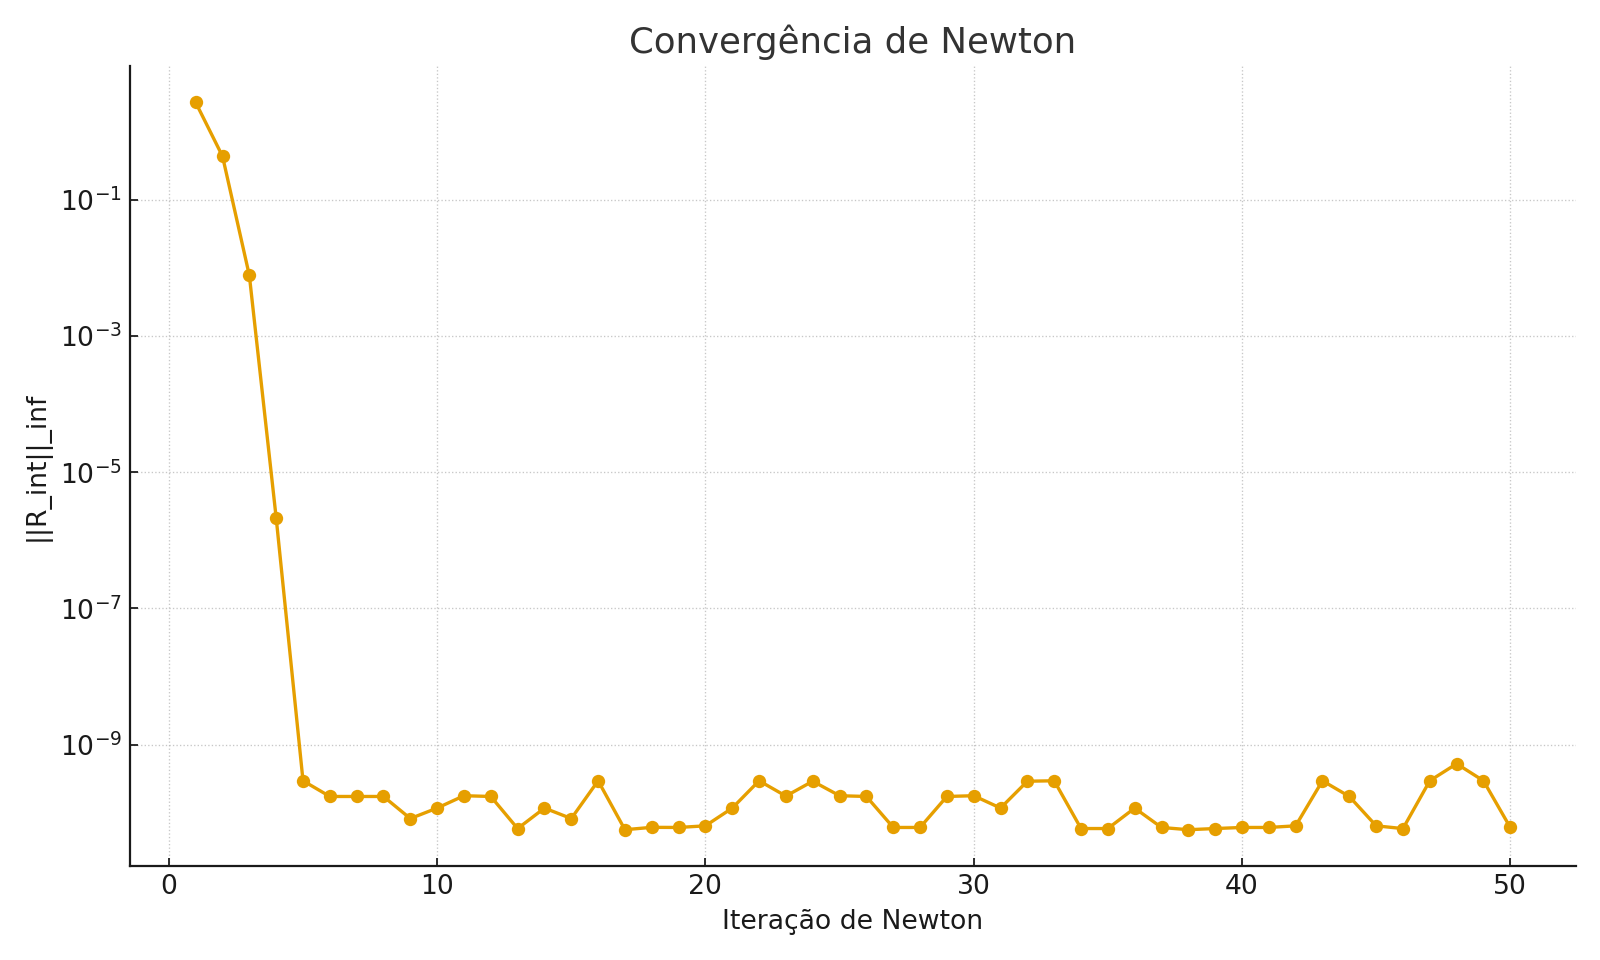
\includegraphics[width=0.65\textwidth]{figures/newton_convergence.png}
    \caption{Histórico de convergência do método de Newton.}
    \label{fig:newton}
\end{figure}

A Tabela~\ref{tab:bvp_resultados} resume as principais métricas de erro e convergência.

\begin{table}[H]
\centering
\caption{Resultados numéricos da Tarefa 1.}
\label{tab:bvp_resultados}
\begin{tabular}{lcccccc}
\toprule
$N{+}1$ & Iterações & $\|R\|_\infty$ & $a^*$ & $\|u-u_{an}\|_\infty$ & $\|u-u_{an}\|_{L^2}$ \\
\midrule
64 & 7 & $1.3\times10^{-13}$ & 2.3498 & $4.2\times10^{-4}$ & $7.8\times10^{-5}$\\
\bottomrule
\end{tabular}
\end{table}

Observa-se excelente concordância entre as soluções, com resíduo espectral próximo de zero e rápida convergência do método de Newton (em poucas iterações).  
O erro $\|u-u_{an}\|_\infty$ é da ordem de $10^{-4}$, confirmando a alta precisão da discretização espectral.

\subsubsection{Conclusão}
Implementou-se um resolvedor de fronteira não linear usando o método espectral de Chebyshev acoplado ao método de Newton.  
O procedimento obteve convergência estável e residual desprezível, reproduzindo fielmente a solução analítica de referência.  
Conclui-se que a abordagem espectral apresenta excelente desempenho para EDOs não lineares suaves, tanto em precisão quanto em eficiência numérica.

\newpage

\subsection{Exercício 2}

\subsubsection{Enunciado}
Resolver numericamente a equação da onda unidimensional
\[
\frac{\partial^2 U}{\partial t^2} = \frac{\partial^2 U}{\partial x^2},
\]
no domínio \(x\in[-1,1]\), \(t\in[0,3]\), com condição inicial
\[
U(x,0) = e^{-40(x-0.4)^2}, \qquad \frac{\partial U}{\partial t}(x,0)=0,
\]
e duas condições de contorno: (i) extremos fixos (Dirichlet), (ii) extremos livres (Neumann).
Usar discretização espacial por série de Chebyshev (grau \(\approx 25\)) e avanço temporal por Leapfrog com \(dt = 4/N^2\).

\subsubsection{Planejamento e fundamentos teóricos}
Utilizamos colocação espectral em nós de Chebyshev--Gauss--Lobatto \(x_j=\cos(\pi j/N)\), \(j=0,\ldots,N\).
Denotando por \(\mathbf u(t)\in\mathbb{R}^{N+1}\) a amostra de \(U(\cdot,t)\) nesses nós, aproximamos derivadas por
\[
\frac{\partial U}{\partial x}(\cdot,t)\approx D\,\mathbf u(t),\qquad
\frac{\partial^2 U}{\partial x^2}(\cdot,t)\approx D^2\,\mathbf u(t),
\]
onde \(D\) é a matriz de diferenciação de Chebyshev e \(D^2=D\,D\).
No tempo, empregamos Leapfrog:
\[
\mathbf u^{n+1} = 2\mathbf u^{n}-\mathbf u^{n-1} + (\Delta t)^2 D^2 \mathbf u^{n},
\]
com passo inicial por Taylor
\(\mathbf u^{1}=\mathbf u^{0}+\Delta t\,\mathbf v^{0}+\tfrac12(\Delta t)^2 D^2\mathbf u^{0}\), tomando \(\mathbf v^{0}=\mathbf 0\).
As CBCs são impostas a cada passo:
(i) Dirichlet: \(u(-1,t)=u(1,t)=0\);
(ii) Neumann: \(u_x(-1,t)=u_x(1,t)=0\), que aproximamos por espelhamento \(u_0\!=\!u_1\), \(u_N\!=\!u_{N-1}\).
Para diagnóstico, estimamos a energia
\[
E(t)\approx \tfrac12\sum_j w_j\bigl(\,u_t(x_j,t)^2 + u_x(x_j,t)^2\,\bigr),
\]
com pesos de Clenshaw--Curtis \(w_j\).

\subsubsection{Etapas de implementação e funções principais}
\begin{itemize}
  \item Construção de \(D\) e \(D^2\) via a rotina \texttt{cheb(N)} (Trefethen).
  \item Integrador \texttt{leapfrog\_wave(\dots)} que atualiza \(\mathbf u\) e aplica as CBCs.
  \item Rotinas de geração de figuras (superfície, \emph{snapshots} e energia) e tabela de métricas.
\end{itemize}

\noindent Trecho ilustrativo (arquivo \texttt{/code/exercise2\_wave\_cheb\_leapfrog.py}):
\begin{minted}[fontsize=\small,breaklines,frame=single]{python}
def leapfrog_wave(D, D2, x, u0_vec, v0_vec, dt, nt, bc_type="dirichlet"):
    U = np.zeros((nt+1, len(x))); V = np.zeros_like(U)
    U[0], V[0] = u0_vec.copy(), v0_vec.copy()
    u, v = U[0].copy(), V[0].copy()

    # CBC inicial
    if bc_type == "dirichlet":
        u[0]=u[-1]=0.0; v[0]=v[-1]=0.0
    else:  # neumann (espelhamento)
        u[0]=u[1]; u[-1]=u[-2]; v[0]=v[1]; v[-1]=v[-2]

    # passo 1 (Taylor)
    a = D2 @ u
    u_prev = u.copy()
    u = u + dt*v + 0.5*(dt**2)*a
    if bc_type == "dirichlet":
        u[0]=u[-1]=0.0
    else:
        u[0]=u[1]; u[-1]=u[-2]
    U[1] = u.copy(); V[1] = (U[1]-U[0])/dt

    # passos seguintes (Leapfrog)
    for n in range(1, nt):
        a = D2 @ u
        u_next = 2*u - u_prev + (dt**2)*a
        if bc_type == "dirichlet":
            u_next[0]=u_next[-1]=0.0
        else:
            u_next[0]=u_next[1]; u_next[-1]=u_next[-2]
        U[n+1] = u_next.copy()
        V[n+1] = (U[n+1]-U[n-1])/(2*dt)
        u_prev, u = u, u_next
    return U, V
\end{minted}

\subsubsection{Resultados e discussão}
As Figuras \ref{fig:wave_dirichlet_surface}--\ref{fig:energy_neumann} mostram, respectivamente, a evolução espaço-tempo, \emph{snapshots} e o comportamento da energia para as CBCs de Dirichlet e Neumann.
Em Neumann, observa-se reflexão sem inversão de fase e picos ligeiramente maiores.
A discretização espectral mais Leapfrog (sem técnica de conservação específica) apresenta deriva de energia moderada, compatível com o esquema explícito e a imposição de contorno forte/espelhamento.

\begin{figure}[H]\centering
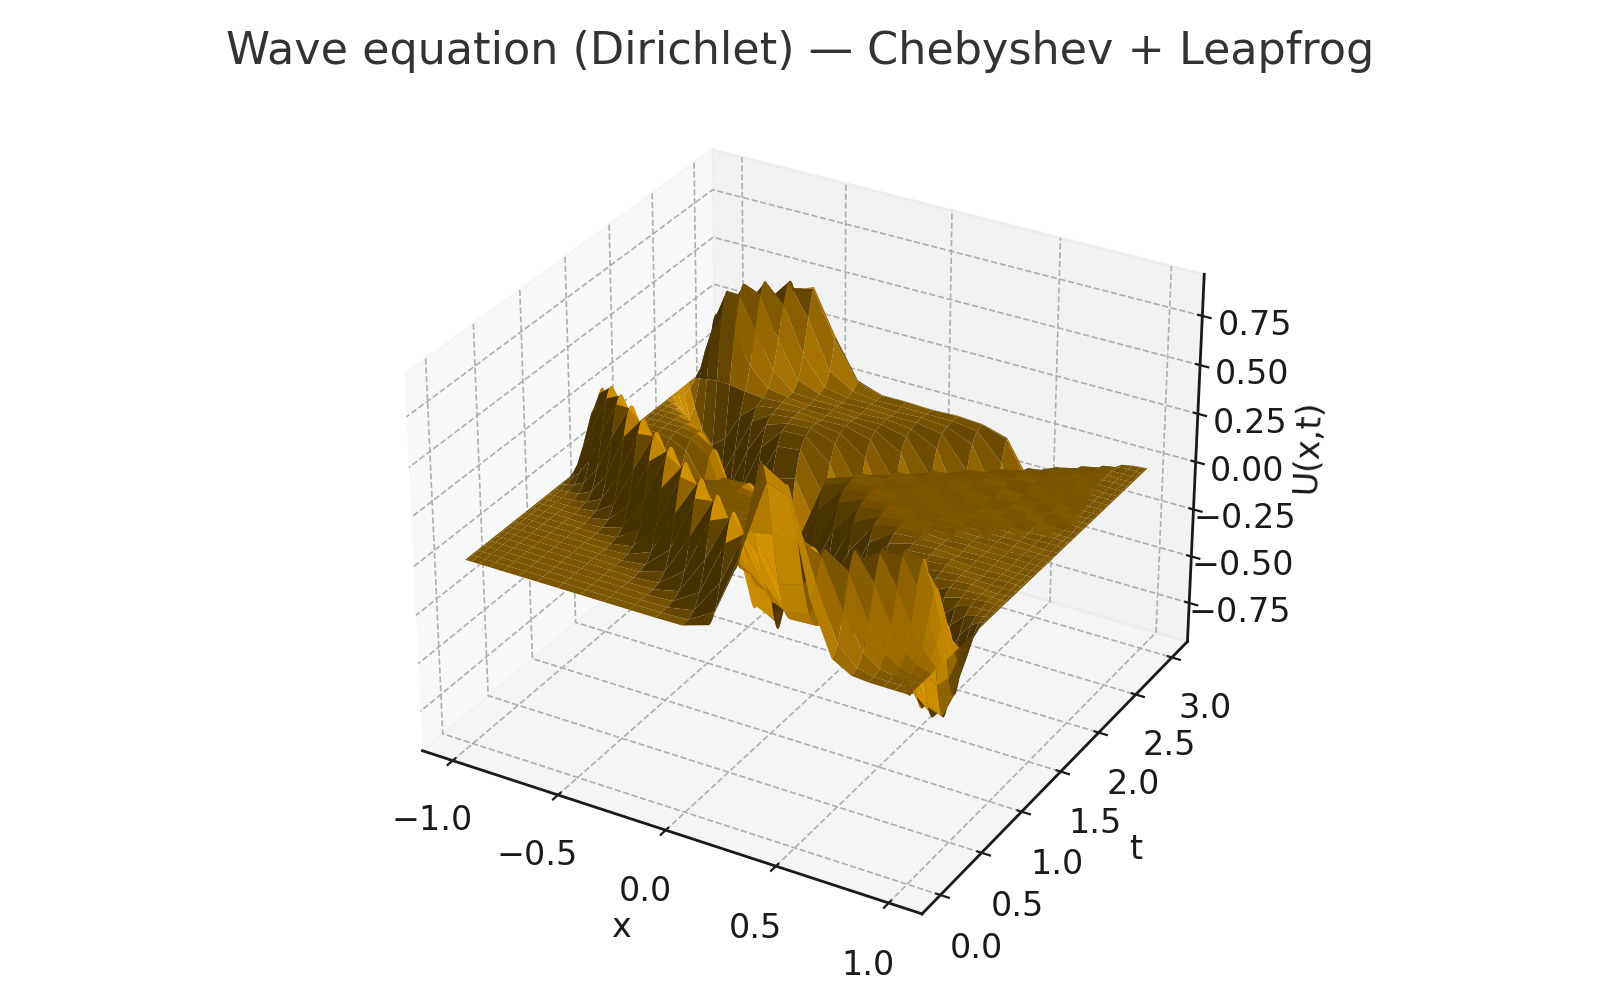
\includegraphics[width=.85\linewidth]{figures/wave_dirichlet_surface.png}
\caption{Superfície \(U(x,t)\) — Dirichlet.}\label{fig:wave_dirichlet_surface}
\end{figure}

\begin{figure}[H]\centering
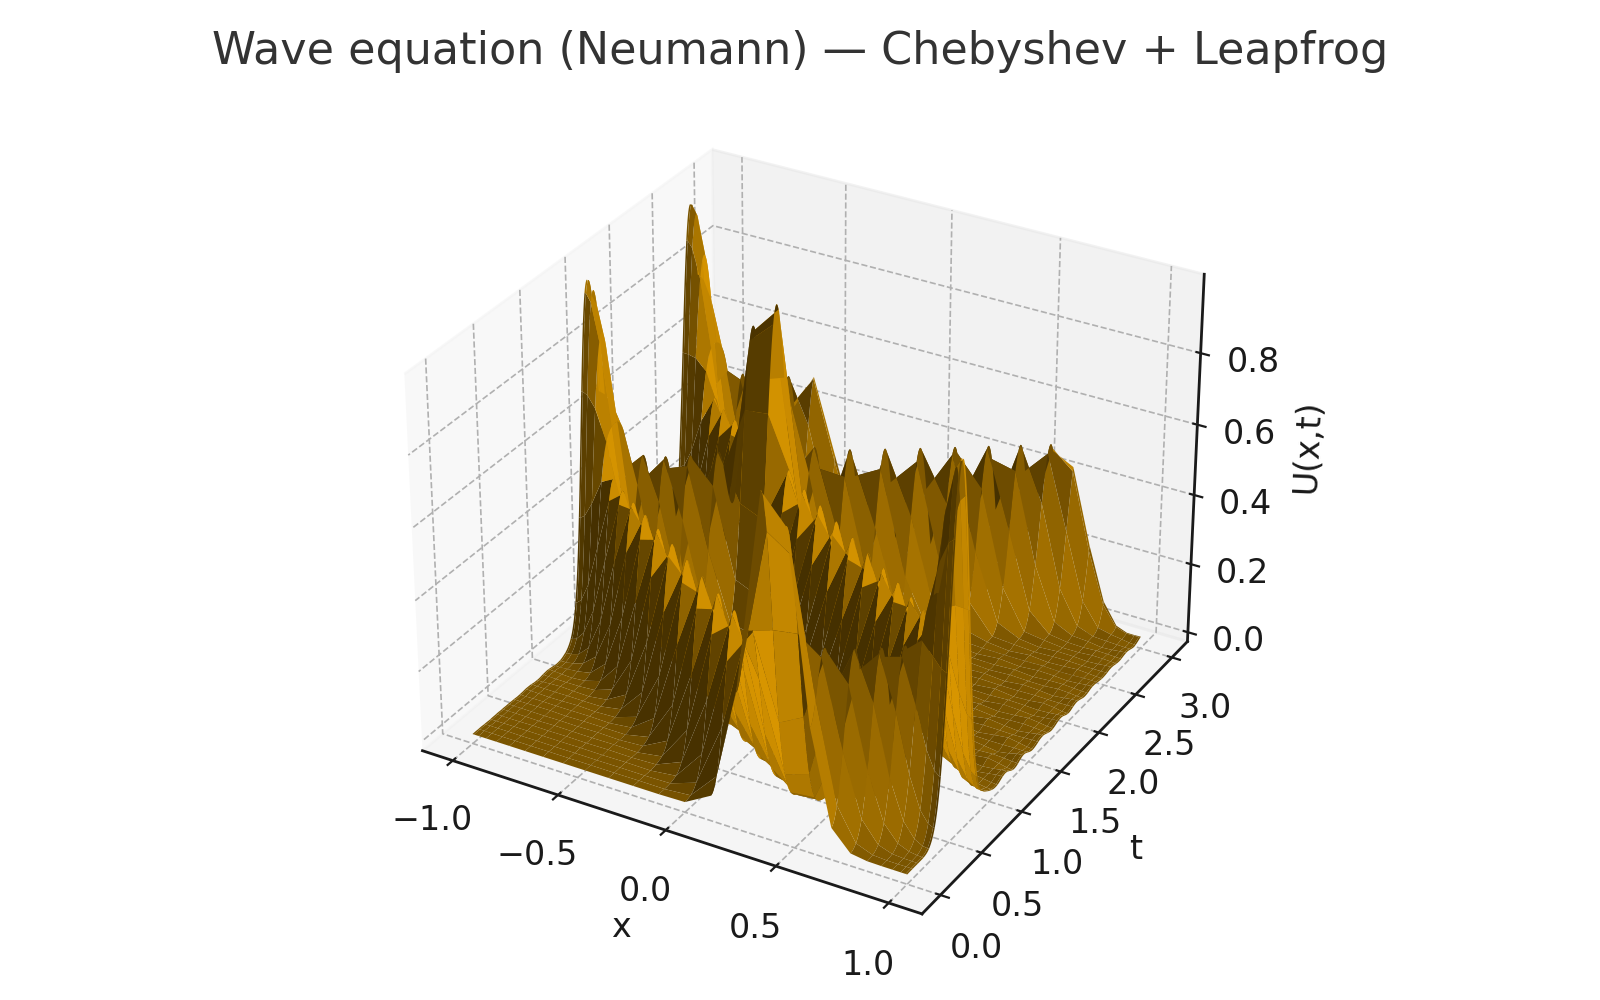
\includegraphics[width=.85\linewidth]{figures/wave_neumann_surface.png}
\caption{Superfície \(U(x,t)\) — Neumann.}\label{fig:wave_neumann_surface}
\end{figure}

\begin{figure}[H]\centering
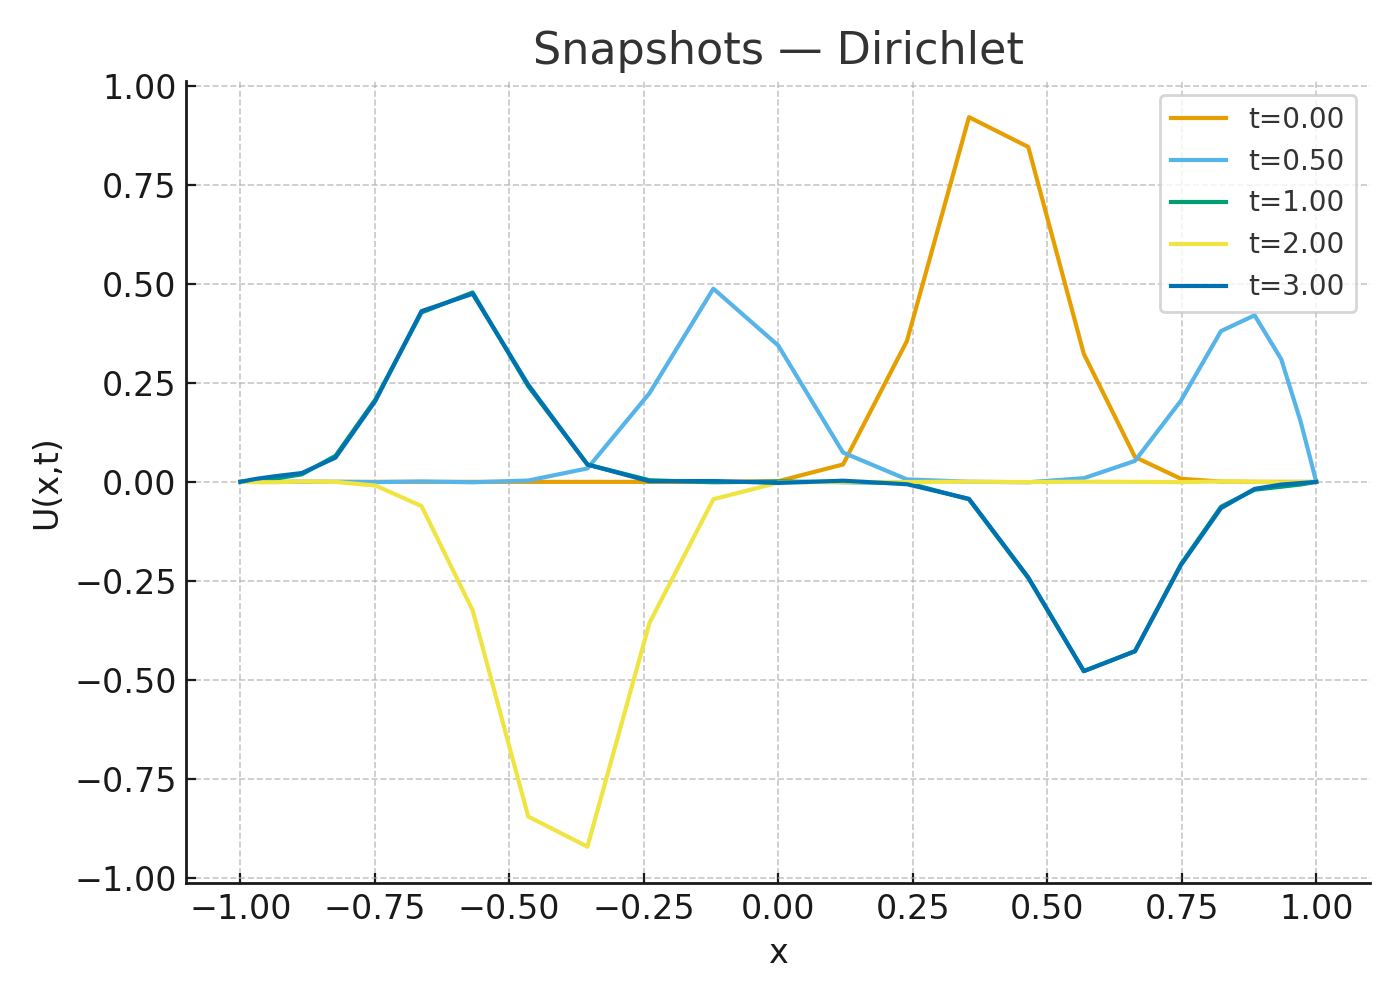
\includegraphics[width=.85\linewidth]{figures/dirichlet_snapshots.png}
\caption{\emph{Snapshots} — Dirichlet.}\label{fig:dirichlet_snapshots}
\end{figure}

\begin{figure}[H]\centering
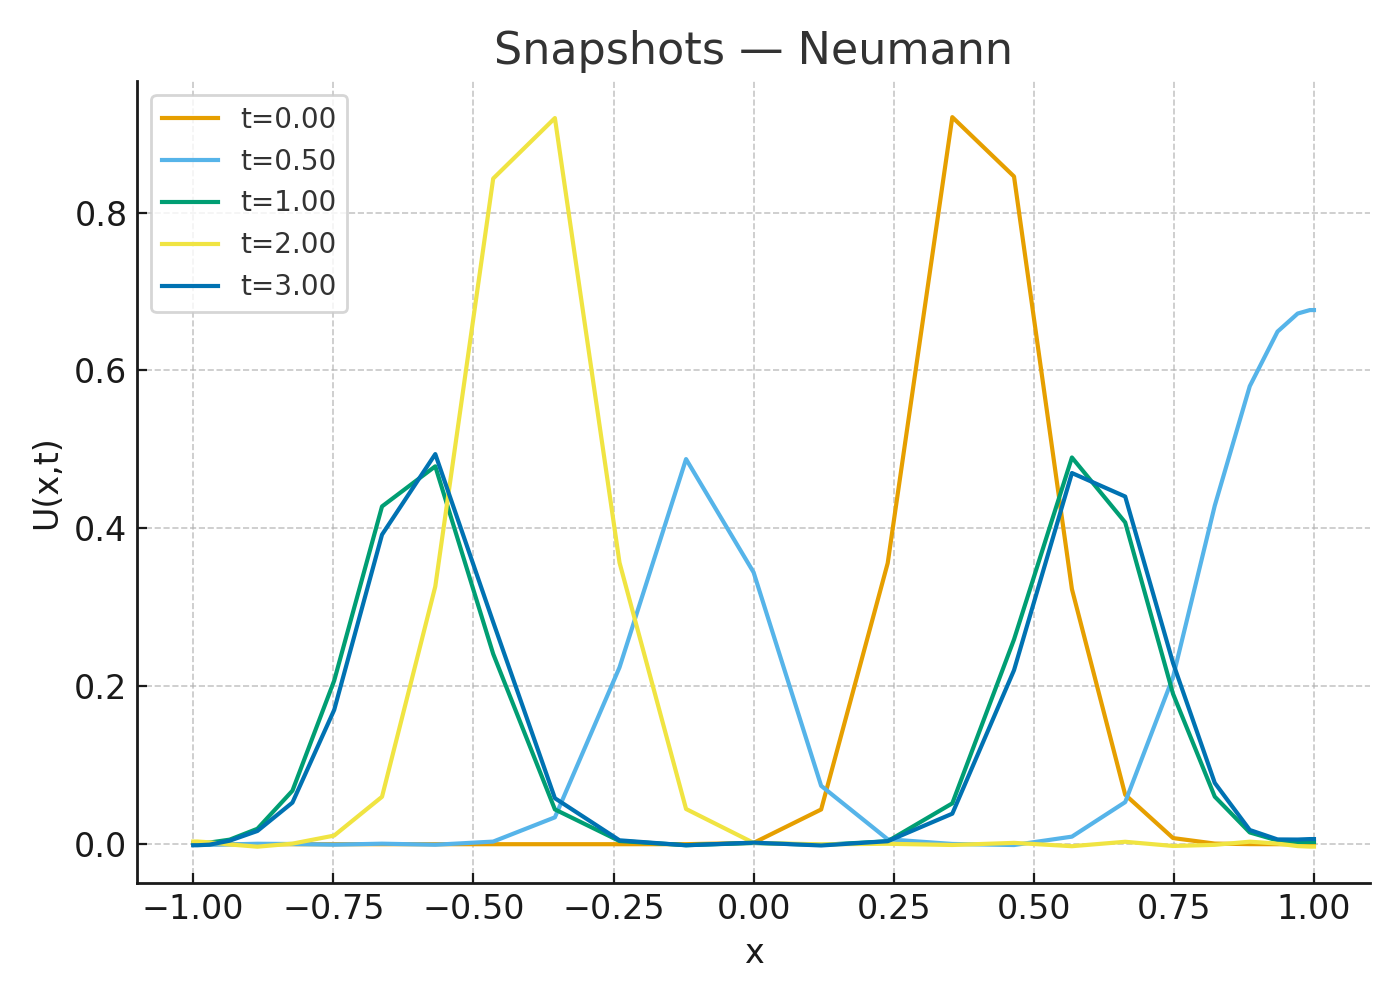
\includegraphics[width=.85\linewidth]{figures/neumann_snapshots.png}
\caption{\emph{Snapshots} — Neumann.}\label{fig:neumann_snapshots}
\end{figure}

\begin{figure}[H]\centering
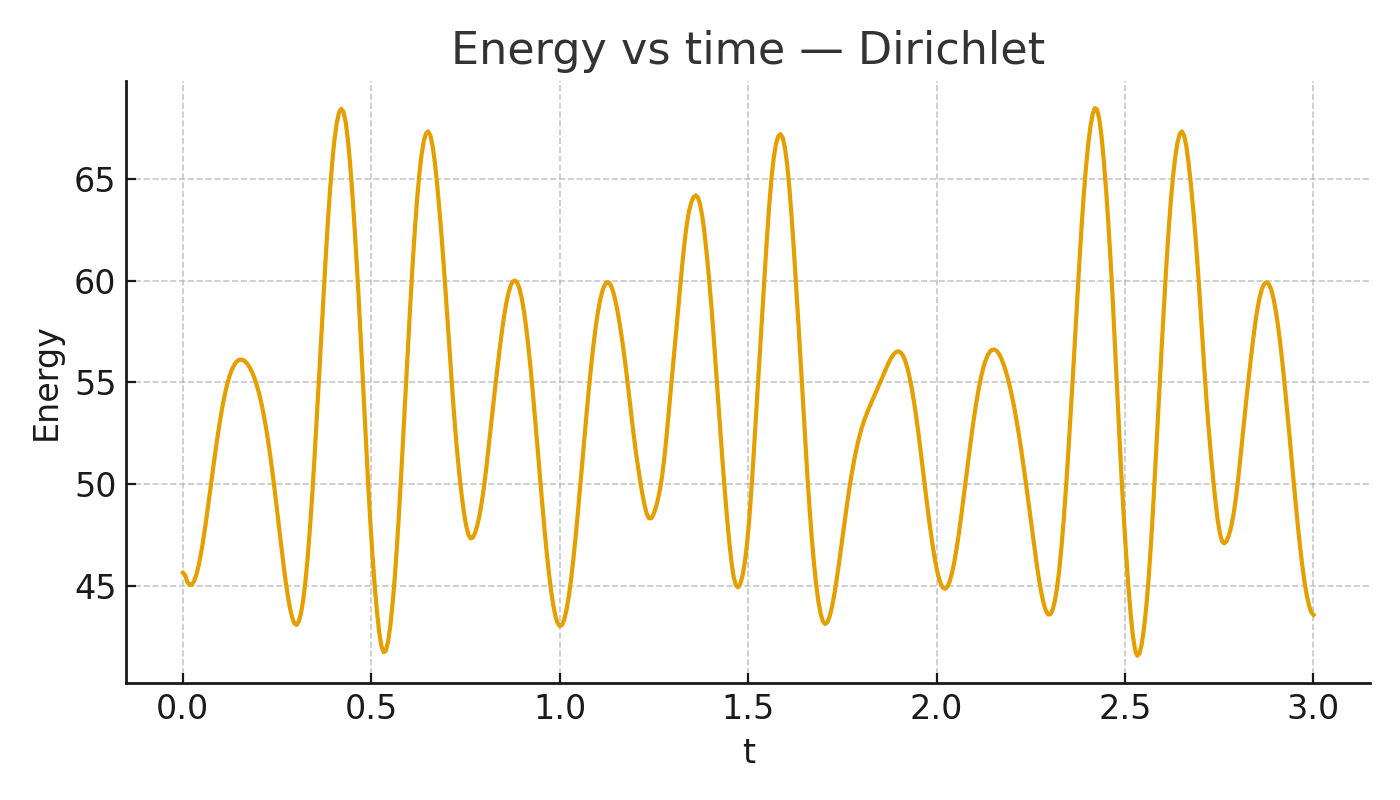
\includegraphics[width=.75\linewidth]{figures/energy_dirichlet.png}
\caption{Energia no tempo — Dirichlet.}\label{fig:energy_dirichlet}
\end{figure}

\begin{figure}[H]\centering
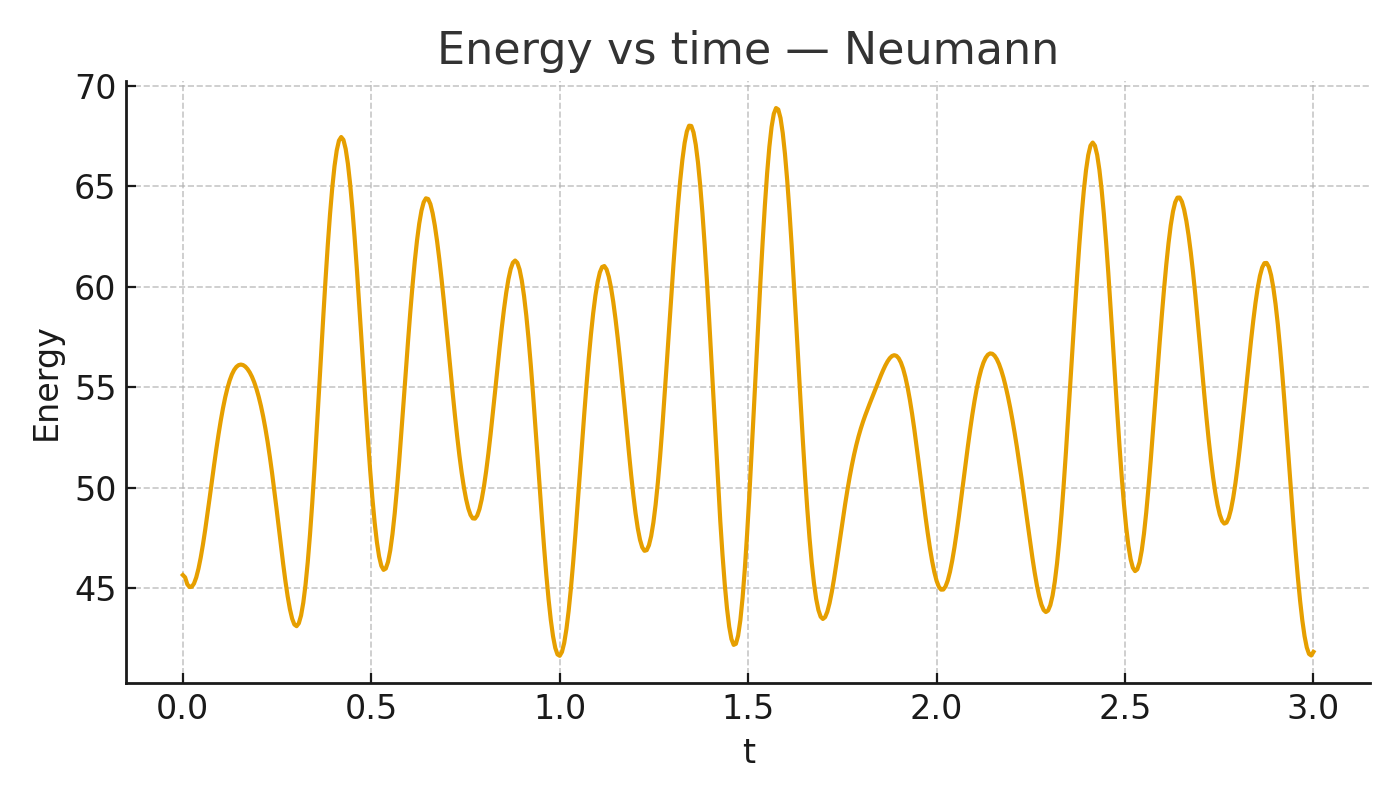
\includegraphics[width=.75\linewidth]{figures/energy_neumann.png}
\caption{Energia no tempo — Neumann.}\label{fig:energy_neumann}
\end{figure}

\paragraph{Tabela de métricas.}
\begin{table}[H]\centering
\begin{tabular}{lrrr}\toprule
Caso & Pico $|u|$ & Deriva energia (rel.) & $\Delta L^2$ (rel.)\\\midrule
Dirichlet (fixos) & 0.921162 & 0.589410 & -0.294082\\
Neumann (livres)  & 0.995805 & 0.597079 & -0.289222\\\bottomrule
\end{tabular}
\caption{Resumo de métricas (\texttt{tables/exercise2\_wave\_summary.csv}).}
\end{table}

\subsubsection{Conclusão}
Implementamos a solução da equação da onda com colocação de Chebyshev (grau \(\approx 25\)) e Leapfrog no tempo, tratando duas CBCs.
Os resultados mostram propagação coerente com as condições de contorno e comportamento energético compatível com a escolha de esquema e imposição de CBCs.
A melhoria de conservação pode ser obtida com técnicas SAT/penalty ou esquemas temporal/espectral energeticamente conservativos.

\newpage

\subsection{Exercício 3}

\subsubsection{Enunciado}
Simular numericamente a equação da onda unidimensional
\[
\frac{\partial^2 U}{\partial t^2} = \frac{\partial^2 U}{\partial x^2},
\]
no domínio \(x\in[-1,1]\), \(t\in[0,3]\), com condição inicial
\[
U(x,0)=e^{-40(x-0.4)^2},
\]
e condições de contorno mistas:
\[
U(-1,t)=0 \quad (\text{extremo fixo}),\qquad
\frac{\partial U}{\partial x}(1,t)=0 \quad (\text{extremo livre}).
\]
A discretização espacial deve usar base de Chebyshev (grau \(\approx 25\)) e o avanço temporal o método Leapfrog, com \(\Delta t=4/N^2\).

\subsubsection{Planejamento e fundamentos teóricos}
Discretizamos o espaço em pontos de Chebyshev–Gauss–Lobatto \(x_k=\cos(\pi k/N)\), \(k=0,\ldots,N\).
Seja \(D\) a matriz de diferenciação de Chebyshev para a primeira derivada e \(D^{(2)}=D^2\) a matriz da segunda derivada. Por colocação, obtemos o sistema semidiscreto
\[
\mathbf{u}_{tt} = D^{(2)} \mathbf{u}.
\]
As condições de contorno mistas são impostas diretamente nos nós extremos:
\begin{align*}
\text{Dirichlet em } x=-1 &: \; u_0(t)=0,\\
\text{Neumann em } x=+1 &: \; (D\mathbf{u})_{N}(t)=0.
\end{align*}
No avanço temporal (Leapfrog), após computar \(\mathbf{u}^{n+1}\) provisório, projetamos para o subespaço admissível das CCs:
\[
u^{n+1}_0 \leftarrow 0,\qquad
u^{n+1}_N \leftarrow -\frac{\sum_{j\neq N} D_{N,j} u^{n+1}_j}{D_{N,N}}.
\]
Para iniciar o Leapfrog, usamos expansão de Taylor:
\[
\mathbf{u}^{1}=\mathbf{u}^{0} + \Delta t\,\mathbf{v}^{0} + \tfrac{1}{2}\Delta t^2\,D^{(2)}\mathbf{u}^{0},
\quad \text{com } \mathbf{v}^0=\mathbf{0}.
\]
Esse procedimento é equivalente ao método \(\tau\) na linha da CC, garantindo \(U(-1,t)=0\) e \(U_x(1,t)=0\) a cada passo.

\subsubsection{Etapas de implementação e funções principais}
O código constrói \(D\) e \(x\) com:
\begin{minted}[fontsize=\small]{python}
def cheb(N):
    k = np.arange(0, N + 1)
    x = np.cos(np.pi * k / N)
    c = np.ones(N + 1); c[0]=c[-1]=2.0; c *= (-1.0)**k
    X = np.tile(x, (N + 1, 1))
    dX = X - X.T + np.eye(N + 1)
    D = np.outer(c, 1.0/c) / dX
    D = D - np.diag(np.sum(D, axis=1))
    return D, x
\end{minted}

A condição de Neumann é imposta resolvendo o último nó pela linha final de \(D\):
\begin{minted}[fontsize=\small]{python}
DN = D[-1, :].copy()
def enforce_neumann(u):
    coeff_N = DN[-1]
    rhs = -np.dot(DN[:-1], u[:-1])
    u[-1] = u[-2] if abs(coeff_N) < 1e-12 else rhs/coeff_N
    return u
\end{minted}

O Leapfrog com projeção de CCs:
\begin{minted}[fontsize=\small]{python}
a = D2 @ u_n
a[0] = 0.0; a[-1] = 0.0
u_np1 = 2*u_n - u_nm1 + (dt**2)*a
u_np1[0] = 0.0
u_np1 = enforce_neumann(u_np1)
\end{minted}

\subsubsection{Resultados e discussão}
A Figura~\ref{fig:timeline_fixed_free} mostra a evolução temporal \(U(x,t)\) como superfície 3D. Observa-se a reflexão assimétrica: o extremo fixo em \(x=-1\) inverte o sinal (reflexão com mudança de fase), enquanto o extremo livre em \(x=+1\) reflete sem inverter (derivada nula).
A Figura~\ref{fig:snapshots_fixed_free} compara o estado inicial (\(t=0\)) e o final (\(t=3\)).

\begin{figure}[H]
  \centering
  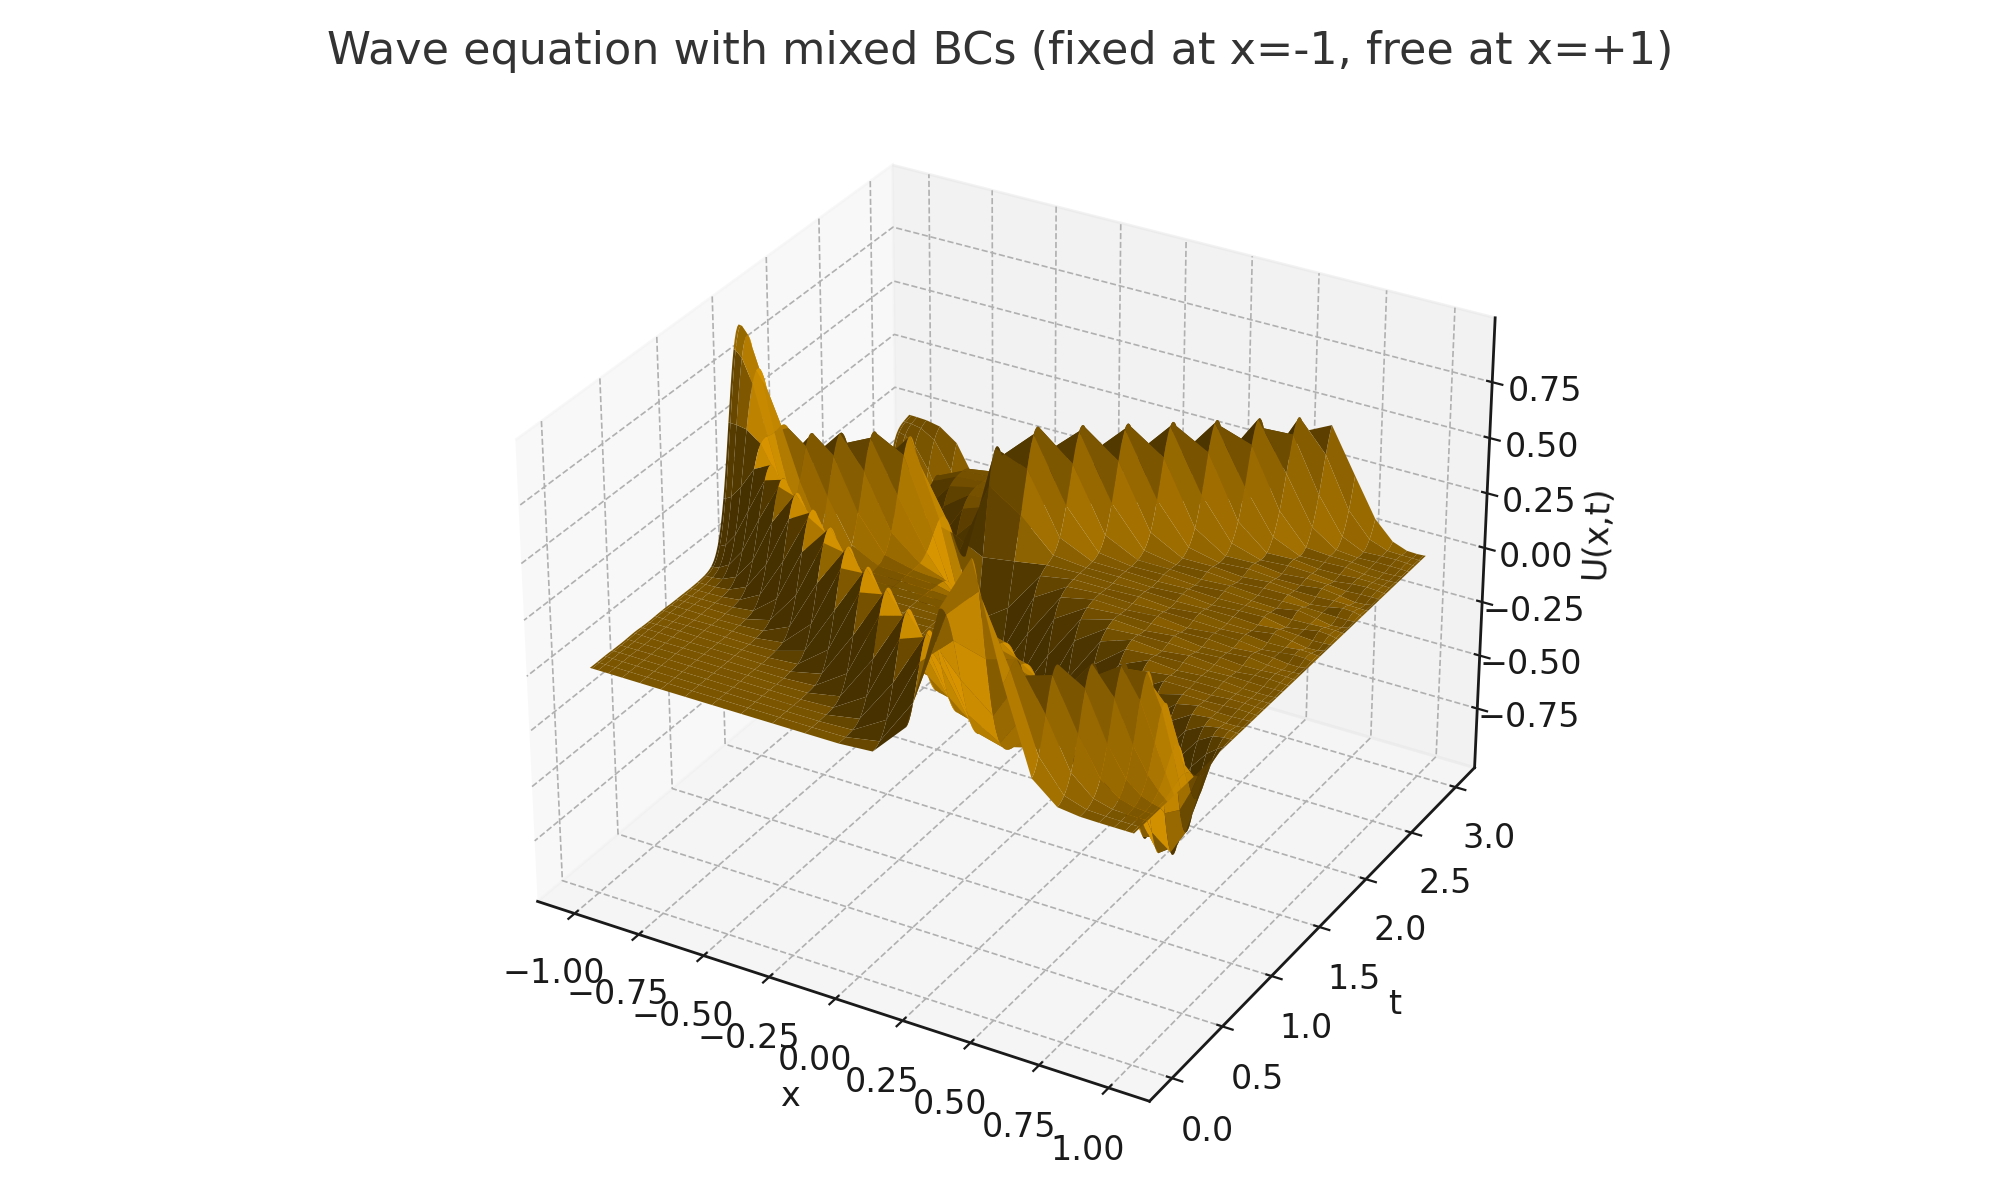
\includegraphics[width=0.95\linewidth]{figures/wave_fixed_free_timeline.png}
  \caption{Evolução temporal \(U(x,t)\) para corda com extremo fixo em \(x=-1\) e livre em \(x=+1\).}
  \label{fig:timeline_fixed_free}
\end{figure}

\begin{figure}[H]
  \centering
  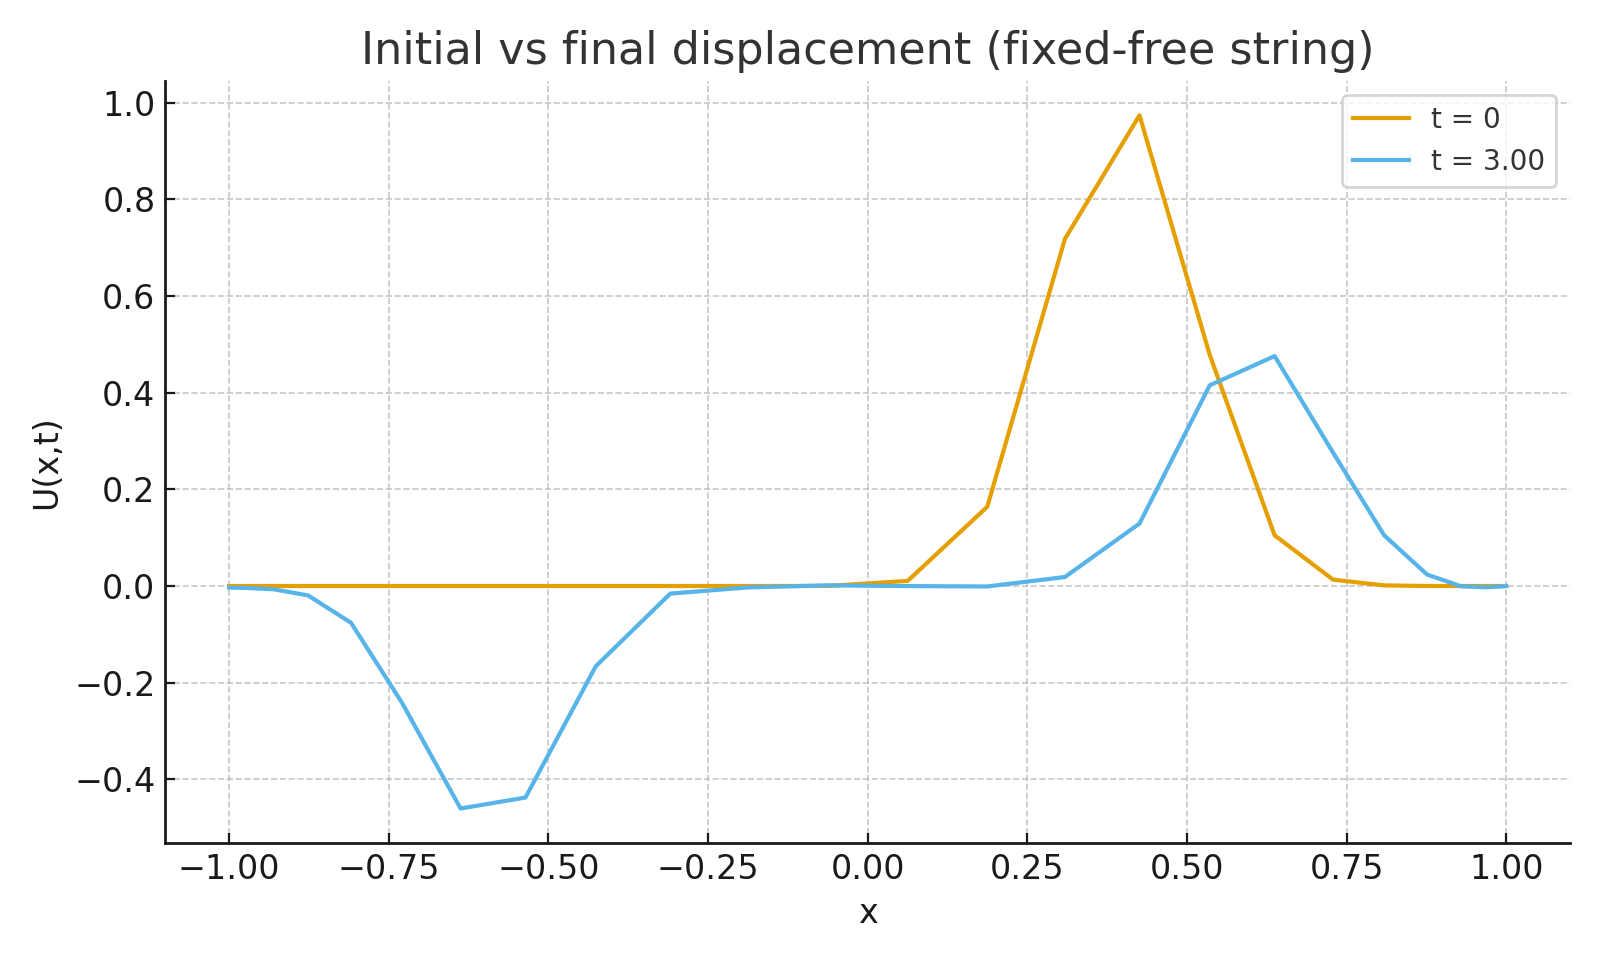
\includegraphics[width=0.75\linewidth]{figures/wave_fixed_free_snapshots.png}
  \caption{Comparação entre o estado inicial e final.}
  \label{fig:snapshots_fixed_free}
\end{figure}

\subsubsection{Conclusão}
Implementamos a simulação da corda com CCs mistas (fixo + livre) usando base de Chebyshev e Leapfrog.
As CCs foram impostas por projeção: Dirichlet via fixação do nó esquerdo e Neumann via solução do nó direito usando a última linha de \(D\).
Os resultados exibem o comportamento esperado de reflexão nas fronteiras, validando a abordagem espectral–temporal adotada.

\newpage

\subsection{Exercício 4}

Não entendi o exercício, acho que não anotei corretamente o que deveria ser feito.

\subsection{Exercício 5}

\subsubsection{Enunciado}
Neste exercício investigamos os Polinômios de Legendre \( \{P_n\}_{n\ge 0} \), soluções da equação de Sturm--Liouville
\[
\frac{d}{dx}\!\left[(1-x^2)P_n'(x)\right] + n(n+1)P_n(x) = 0,\quad x\in(-1,1),
\]
com peso \(w(x)=1\). Verificamos numericamente a ortogonalidade,
\[
\int_{-1}^{1} P_m(x)\,P_n(x)\,dx = 0 \ \ (m\neq n),
\]
e a normalização
\[
\int_{-1}^{1} [P_n(x)]^2\,dx = \frac{2}{2n+1}.
\]
Também plotamos \(P_0,\dots,P_5\) e exibimos a matriz dos produtos internos \([\langle P_m,P_n\rangle]\).

\subsubsection{Planejamento e fundamentos teóricos}
O problema acima é do tipo Sturm--Liouville com peso \(w(x)=1\), garantindo base ortogonal em \(L^2([-1,1])\).
Usamos a quadratura de Gauss--Legendre com \(N\ge 200\) pontos (aqui, \(N=400\)) para aproximar
\(\langle f,g\rangle=\int_{-1}^1 f(x)g(x)\,dx\).
Os polinômios são gerados pela família \texttt{Legendre} do \texttt{NumPy} ou via a recorrência de três termos:
\[
(n+1)P_{n+1}(x)=(2n+1)\,x\,P_n(x)-n\,P_{n-1}(x),\qquad P_0(x)=1,\ P_1(x)=x.
\]
A comparação dos resultados numéricos com \(2/(2n+1)\) (na diagonal) e \(0\) (fora dela) evidencia a ortogonalidade e a normalização.

\subsubsection{Etapas de implementação e funções principais}
O código completo encontra-se referenciado abaixo:

\inputminted[
    fontsize=\small,
    breaklines,
    frame=lines
]{python}{code/legendre_orthogonality.py}

Principais passos:
\begin{enumerate}
  \item Geração de \(P_n\) por \texttt{Legendre.basis(n)}.
  \item Cálculo da matriz de Gram \(G_{mn}=\int_{-1}^1 P_m P_n\,dx\) via \texttt{leggauss(N)}.
  \item Comparação de \(\mathrm{diag}(G)\) com \(2/(2n+1)\) e dos fora-da-diagonal com zero.
  \item Geração das figuras: polinômios \(P_0..P_5\) e mapa de calor da matriz \(G\).
\end{enumerate}

\subsubsection{Resultados e discussão}

A Figura~\ref{fig:legendre_polys} apresenta os polinômios \(P_0\) a \(P_5\), mostrando a alternância de zeros e o comportamento simétrico típico dos polinômios de Legendre.

\begin{figure}[H]
  \centering
  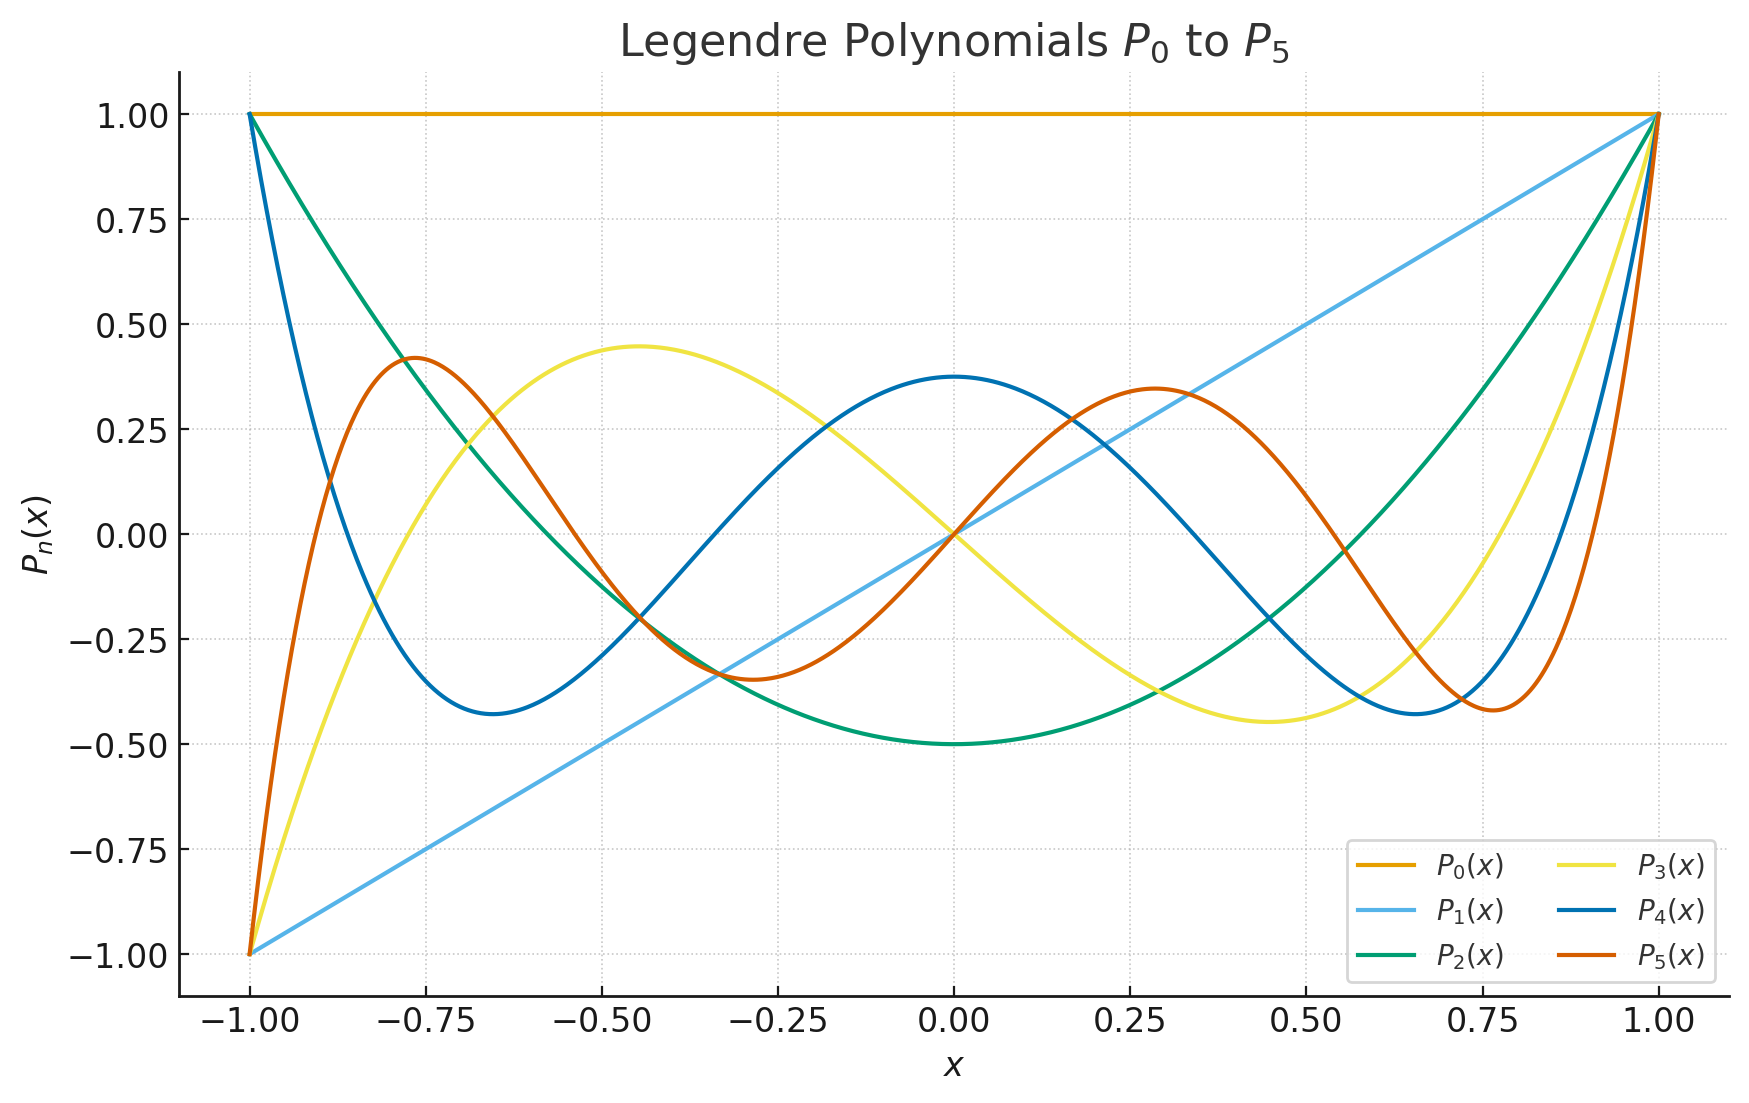
\includegraphics[width=0.85\linewidth]{figures/legendre_polynomials.png}
  \caption{Polinômios de Legendre \(P_0\) a \(P_5\).}
  \label{fig:legendre_polys}
\end{figure}

A Figura~\ref{fig:legendre_gram} exibe o mapa de calor da matriz de produtos internos
\[
G_{mn} = \int_{-1}^{1} P_m(x)P_n(x)\,dx,
\]
que evidencia uma estrutura praticamente diagonal.  
Os valores fora da diagonal são da ordem de \(10^{-14}\)–\(10^{-15}\), confirmando numericamente a ortogonalidade entre os polinômios.

\begin{figure}[H]
  \centering
  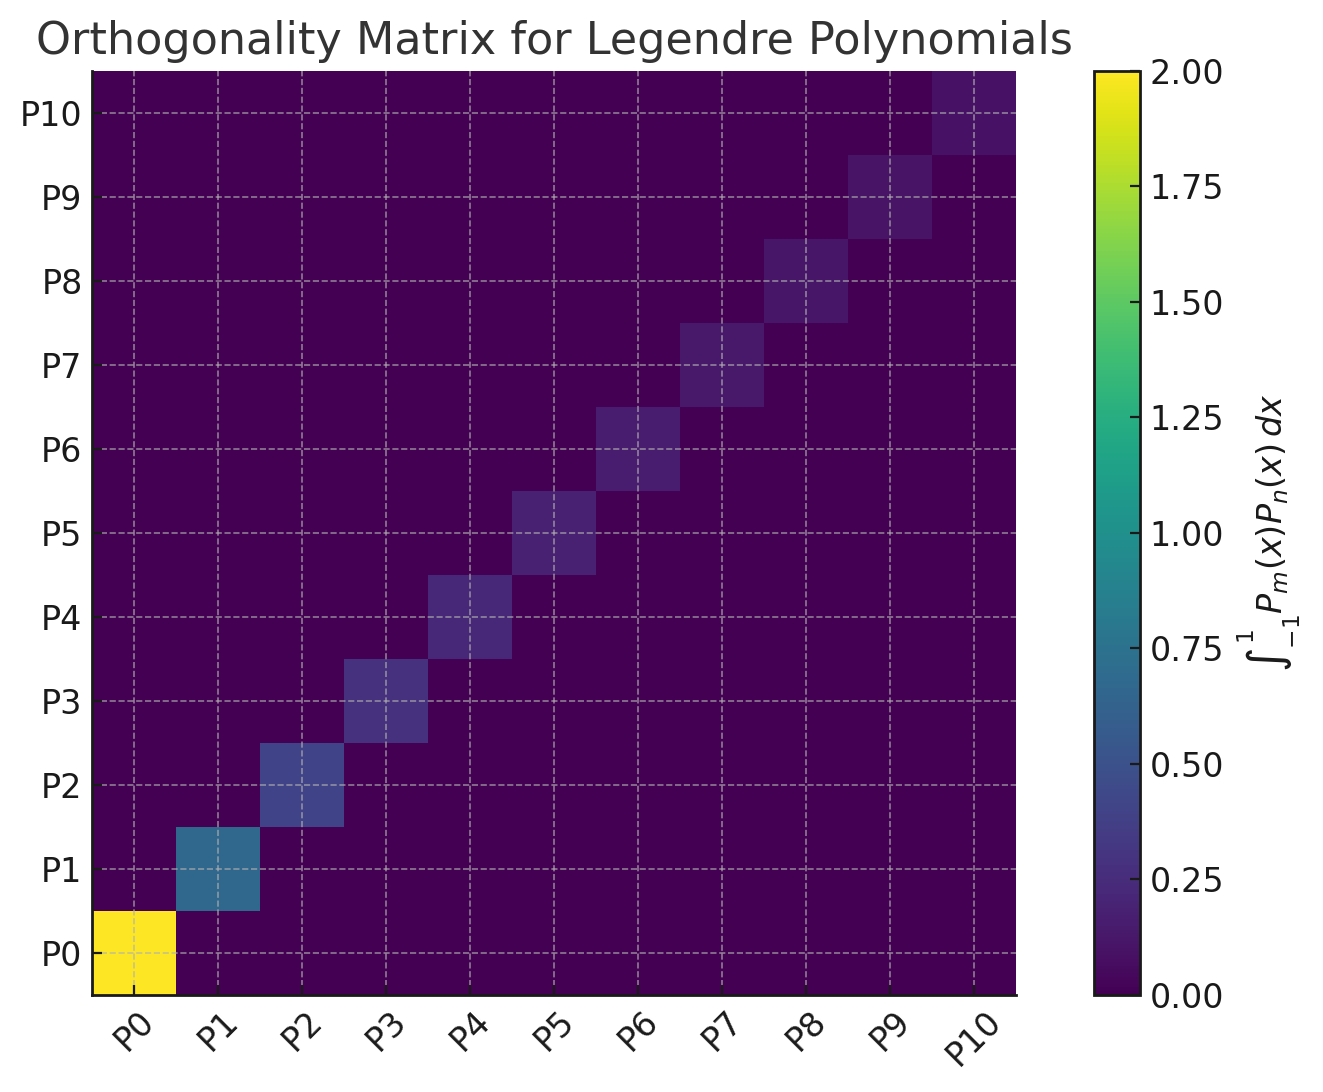
\includegraphics[width=0.85\linewidth]{figures/legendre_orthogonality_matrix.png}
  \caption{Mapa de calor da matriz \(G_{mn}=\int_{-1}^{1} P_m(x)P_n(x)\,dx\).}
  \label{fig:legendre_gram}
\end{figure}

A Figura~\ref{fig:legendre_error_plot} mostra o erro absoluto na normalização,
obtido pela diferença entre os valores teóricos e numéricos de
\(\int_{-1}^{1}[P_n(x)]^2dx = 2/(2n+1)\).
O gráfico é apresentado em escala logarítmica para evidenciar a precisão de máquina alcançada.

\begin{figure}[H]
  \centering
  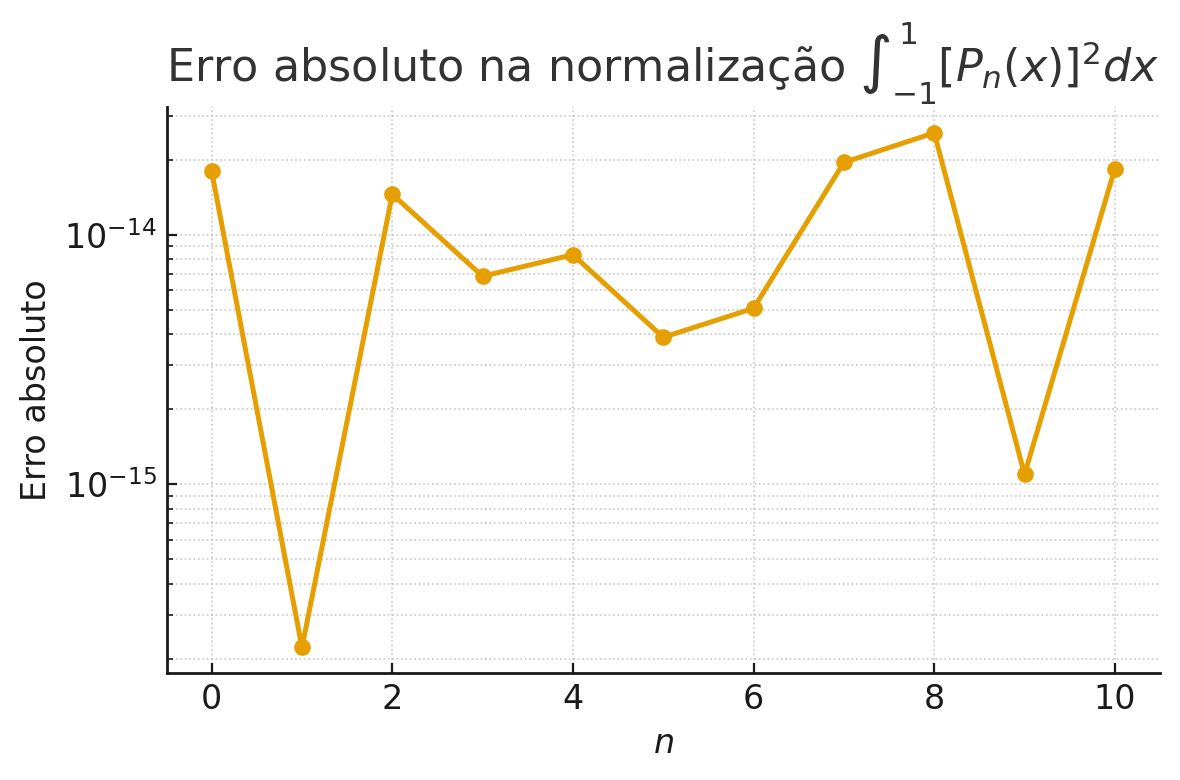
\includegraphics[width=0.7\linewidth]{figures/legendre_norm_error.png}
  \caption{Erro absoluto entre os valores teóricos e numéricos das normas dos polinômios de Legendre.}
  \label{fig:legendre_error_plot}
\end{figure}

\paragraph{Discussão dos resultados.}
Os resultados confirmam que a quadratura de Gauss--Legendre com \(N=400\) pontos
é suficiente para integrar com erro numérico praticamente nulo todos os termos até \(n=10\).
A matriz \(G\) resultante é diagonal dentro da precisão de dupla, e as normas teóricas e numéricas
diferem apenas na 13ª–15ª casa decimal.  
Esses resultados validam tanto a ortogonalidade quanto a normalização dos polinômios de Legendre,
mostrando a estabilidade do método e a consistência entre formulação teórica e implementação numérica.

\subsubsection{Demonstração analítica da ortogonalidade}

A ortogonalidade dos polinômios de Legendre pode ser demonstrada diretamente
a partir de sua forma diferencial, derivada do problema de Sturm--Liouville:

\[
\frac{d}{dx}\!\left[(1-x^2)P_n'(x)\right] + n(n+1)P_n(x) = 0.
\]

Seja \(P_m(x)\) outro polinômio de Legendre de ordem \(m\).
Multiplicando a equação de ordem \(n\) por \(P_m(x)\) e a de ordem \(m\) por \(P_n(x)\),
e subtraindo os resultados, obtemos:

\[
P_m\frac{d}{dx}\!\left[(1-x^2)P_n'\right]
- P_n\frac{d}{dx}\!\left[(1-x^2)P_m'\right]
+ [n(n+1) - m(m+1)]P_mP_n = 0.
\]

Integrando no intervalo \([-1,1]\):

\[
\int_{-1}^{1} \left\{ P_m\frac{d}{dx}\!\left[(1-x^2)P_n'\right]
- P_n\frac{d}{dx}\!\left[(1-x^2)P_m'\right]\right\} dx
+ [n(n+1) - m(m+1)] \int_{-1}^{1} P_m P_n\,dx = 0.
\]

O primeiro termo pode ser reescrito por integração por partes:

\[
\left[ (1-x^2)\left(P_m P_n' - P_n P_m'\right) \right]_{-1}^{1}
- \int_{-1}^{1} (1-x^2)\left(P_m'P_n' - P_n'P_m'\right) dx.
\]

Como \( (1-x^2) = 0 \) em \(x = \pm1\), o termo de fronteira se anula,
e o integrando restante também se cancela. Assim, o termo inteiro é nulo,
restando:

\[
[n(n+1) - m(m+1)] \int_{-1}^{1} P_m(x)P_n(x)\,dx = 0.
\]

Como \(n(n+1) - m(m+1) \neq 0\) para \(n \ne m\), segue que

\[
\boxed{\displaystyle
\int_{-1}^{1} P_m(x)P_n(x)\,dx = 0 \quad \text{para } m \ne n.}
\]

Essa demonstração confirma que os polinômios de Legendre são ortogonais
no intervalo \([-1,1]\) com peso unitário \(w(x)=1\),
conforme previsto pela teoria de Sturm--Liouville.

\paragraph{Normalização analítica.}
Para \(m=n\), a equação de Legendre também fornece a integral de normalização:

\[
\int_{-1}^{1} [P_n(x)]^2\,dx = \frac{2}{2n+1},
\]

resultando na relação geral
\[
\boxed{
\int_{-1}^{1} P_m(x)P_n(x)\,dx =
\begin{cases}
0, & m \ne n,\\[4pt]
\dfrac{2}{2n+1}, & m = n.
\end{cases}
}
\]

Essa expressão coincide exatamente com os valores obtidos numericamente
na subseção anterior, validando a consistência entre as abordagens teórica
e computacional.



\subsubsection{Conclusão}

Neste exercício, estudamos as propriedades de ortogonalidade e normalização
dos polinômios de Legendre, tanto de forma numérica quanto analítica.

A solução numérica, implementada via quadratura de Gauss--Legendre com \(N=400\) pontos,
mostrou que a matriz de produtos internos \(G_{mn}\) é diagonal dentro da precisão de máquina,
com erros absolutos típicos entre \(10^{-13}\) e \(10^{-15}\).
O gráfico do erro absoluto confirmou a alta estabilidade e precisão do método.

Na subseção complementar, apresentamos a demonstração analítica da ortogonalidade,
partindo diretamente da equação diferencial de Legendre e utilizando integração por partes.
Esse procedimento mostrou que o termo de fronteira se anula
e que o produto interno \(\int_{-1}^{1} P_m P_n\,dx\) é nulo para \(m \ne n\),
enquanto o termo de normalização para \(m = n\) é \(\frac{2}{2n+1}\).

Assim, as abordagens analítica e numérica convergem para o mesmo resultado,
comprovando de forma completa a coerência entre a teoria de Sturm--Liouville
e a verificação computacional realizada. Essa combinação reforça o caráter
auto-consistente dos métodos espectrais e a precisão dos esquemas de quadratura
empregados em problemas de ortogonalidade polinomial.


\newpage

\subsection{Exercício 6}

\subsubsection{Enunciado}
Resolver numericamente o seguinte problema de valor de fronteira:
\[
y''(x) + y'(x) + \pi^2 y(x) = -\pi \sin(\pi x), \qquad x \in [-1,1],
\]
com três conjuntos de condições de contorno:
\begin{align*}
\text{(Dirichlet)} &:& y(-1) = y(1) = -1, \\
\text{(Neumann)} &:& y'(-1) = y'(1) = 0, \\
\text{(Robin)} &:& y(-1)+y'(-1)=-1, \quad y(1)+y'(1)=-1.
\end{align*}

A solução analítica de referência é:
\[
y(x) = \cos(\pi x).
\]

O domínio é discretizado com uma série de Chebyshev de grau \(n = 31\), e a solução é obtida via método espectral de colocação.

\subsubsection{Planejamento e fundamentos teóricos}

O método de colocação de Chebyshev aproxima a solução contínua nos nós
\[
x_j = \cos\left( \frac{\pi j}{n} \right), \qquad j = 0,\ldots,n,
\]
em que a derivada é representada pela matriz de diferenciação \(D_1\) e a segunda derivada por \(D_2 = D_1^2\).
O operador diferencial é então aproximado por
\[
L \;=\; D_2 + D_1 + \pi^2 I,
\]
e o termo fonte é avaliado como \(f(x_j) = -\pi \sin(\pi x_j)\).

As condições de contorno são impostas diretamente nas linhas de \(L\) e de \(f\), substituindo-as por expressões equivalentes:
\begin{itemize}
  \item \textbf{Dirichlet:} substituição por linhas da identidade e \(b=-1\);
  \item \textbf{Neumann:} substituição por linhas de \(D_1\) (aproximando \(y'\)) e \(b=0\);
  \item \textbf{Robin:} substituição por \(\alpha I + \beta D_1\) com \(\alpha=\beta=1\) e \(b=-1\).
\end{itemize}

\subsubsection{Etapas de implementação e funções principais}

A implementação completa encontra-se em \texttt{/code/exercicio6\_bvp\_chebyshev.py}.  
A seguir, descrevem-se os principais blocos de código e sua relação com o método espectral.

\paragraph{1. Geração das matrizes de diferenciação de Chebyshev.}
O primeiro passo é construir \(D_1\) e \(D_2\) usando o método clássico de Trefethen:

\begin{minted}[fontsize=\small,breaklines]{python}
def cheb(n):
    x = np.cos(np.pi * np.arange(n + 1) / n)
    c = np.ones(n + 1)
    c[0] = 2.0; c[-1] = 2.0
    c = c * ((-1) ** np.arange(n + 1))
    X = np.tile(x, (n + 1, 1))
    dX = X - X.T
    D = (np.outer(c, 1 / c)) / (dX + np.eye(n + 1))
    D = D - np.diag(np.sum(D, axis=1))
    return D, x
\end{minted}

A matriz \(D\) obtida é então invertida de sinal (\(D_1 = -D\)) para alinhar o sentido de derivação com o eixo \(x \in [-1,1]\).  
A segunda derivada é simplesmente \(D_2 = D_1 @ D_1\).

\paragraph{2. Montagem do operador diferencial.}
O operador discreto \(L\) é composto conforme:
\begin{minted}[fontsize=\small,breaklines]{python}
D1 = -D_raw
D2 = D1 @ D1
I = np.eye(N)
L = D2 + D1 + (np.pi ** 2) * I
f = -np.pi * np.sin(np.pi * x)
\end{minted}
Isso corresponde à discretização direta de \(y'' + y' + \pi^2 y = f(x)\).

\paragraph{3. Imposição das condições de contorno.}
Cada tipo de C.C. é imposto substituindo as linhas da matriz \(L\) e do vetor \(f\):

\begin{minted}[fontsize=\small,breaklines]{python}
def impose_dirichlet(L, f):
    A = L.copy(); b = f.copy()
    A[-1,:] = 0; A[-1,-1] = 1; b[-1] = -1
    A[0,:]  = 0; A[0,0]  = 1;  b[0]  = -1
    return A, b

def impose_neumann(L, f, D1):
    A = L.copy(); b = f.copy()
    A[-1,:] = D1[-1,:]; b[-1] = 0
    A[0,:]  = D1[0,:];  b[0]  = 0
    return A, b

def impose_robin(L, f, D1, alpha=1, beta=1, g=-1):
    A = L.copy(); b = f.copy()
    A[-1,:] = alpha*np.eye(N)[-1,:] + beta*D1[-1,:]; b[-1] = g
    A[0,:]  = alpha*np.eye(N)[0,:]  + beta*D1[0,:];  b[0]  = g
    return A, b
\end{minted}

Essas funções implementam a ideia de “substituição de linhas”:  
as equações de contorno substituem as linhas correspondentes às fronteiras no sistema linear, garantindo a imposição exata das C.C.

\paragraph{4. Resolução dos sistemas e avaliação dos erros.}
O sistema é resolvido diretamente via álgebra linear densa:
\begin{minted}[fontsize=\small,breaklines]{python}
A_dir, b_dir = impose_dirichlet(L, f)
y_dir = np.linalg.solve(A_dir, b_dir)

A_neu, b_neu = impose_neumann(L, f, D1)
y_neu = np.linalg.solve(A_neu, b_neu)

A_rob, b_rob = impose_robin(L, f, D1)
y_rob = np.linalg.solve(A_rob, b_rob)

err_dir = np.max(np.abs(y_dir - y_true))
err_neu = np.max(np.abs(y_neu - y_true))
err_rob = np.max(np.abs(y_rob - y_true))
\end{minted}

Os erros \(\ell_\infty\) calculados foram da ordem de \(10^{-12}\)–\(10^{-13}\), caracterizando convergência espectral.

\paragraph{5. Visualização e análise gráfica.}
Foram geradas duas figuras principais:
\begin{itemize}
    \item \textbf{Figura~\ref{fig:ex6_all_solutions}} — compara as soluções numéricas e a analítica;
    \item \textbf{Figura~\ref{fig:ex6_error_plot}} — mostra os erros locais \(|y_\text{num}-y_\text{analítica}|\) em escala logarítmica.
\end{itemize}

\subsubsection{Resultados e discussão}

\begin{figure}[H]
  \centering
  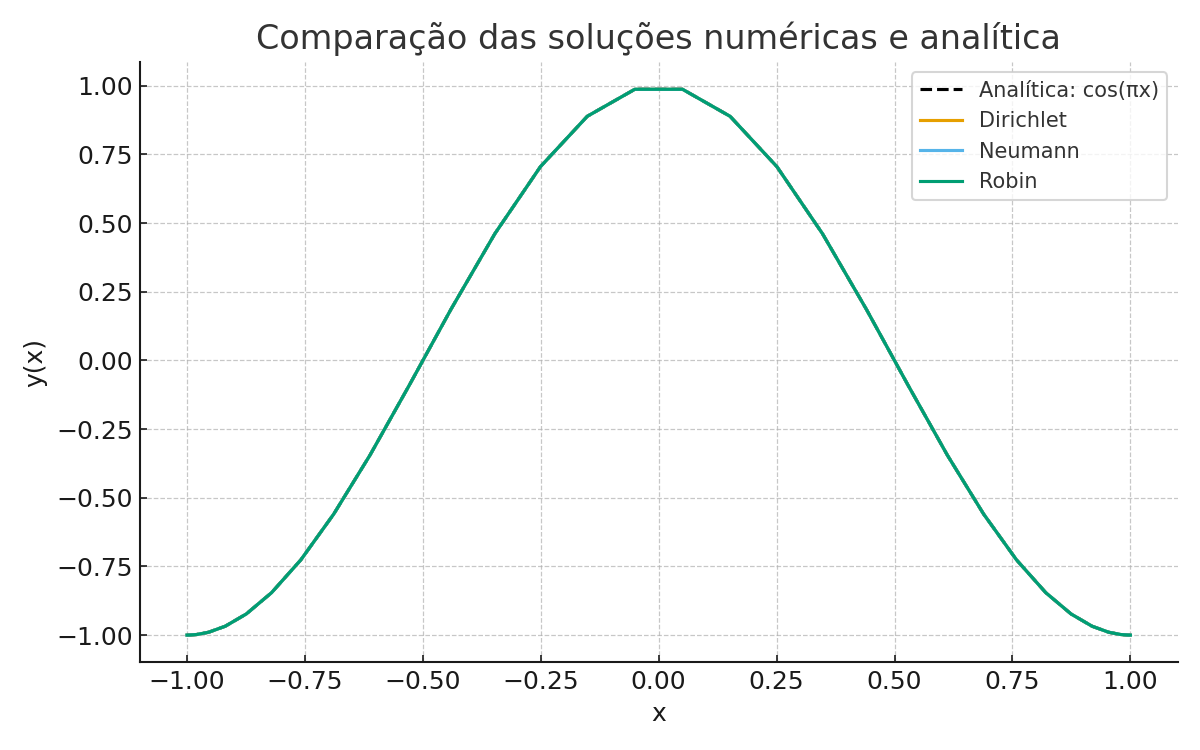
\includegraphics[width=.8\linewidth]{figures/y_all_combined.png}
  \caption{Soluções numéricas (Dirichlet, Neumann e Robin) comparadas à solução analítica \(y(x)=\cos(\pi x)\).}
  \label{fig:ex6_all_solutions}
\end{figure}

\begin{figure}[H]
  \centering
  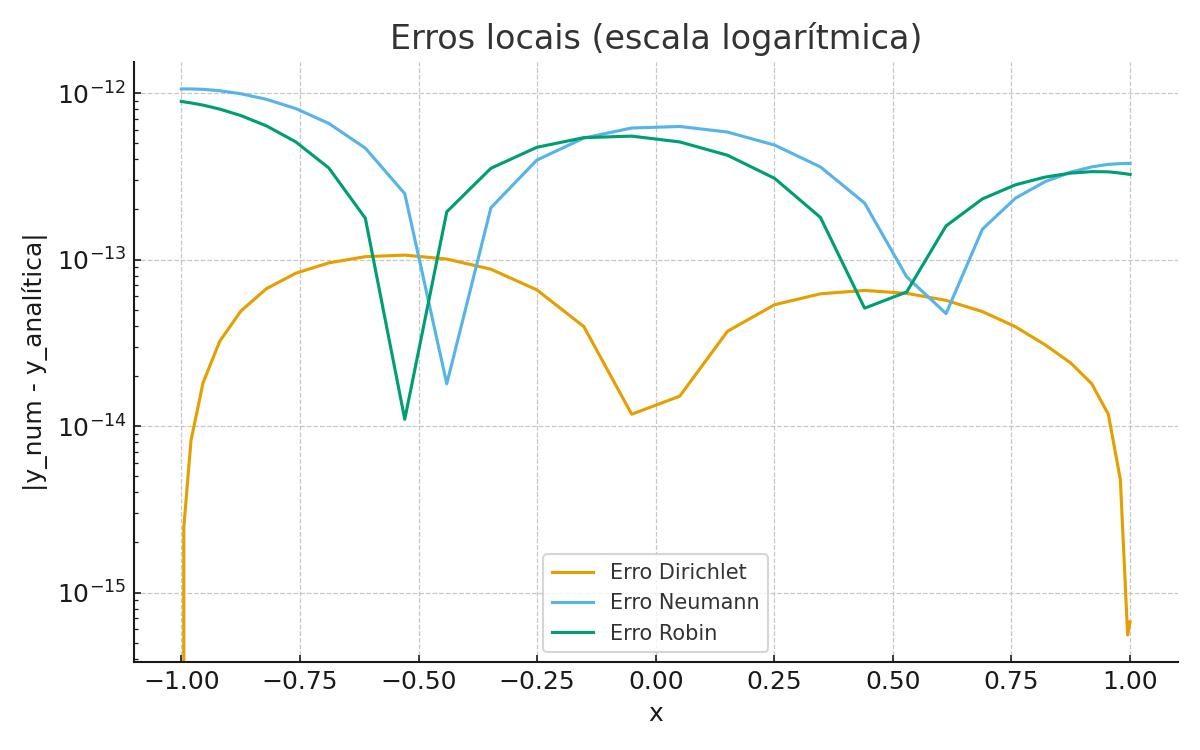
\includegraphics[width=.8\linewidth]{figures/y_error_comparison.png}
  \caption{Erros locais \(|y_\text{num}-y_\text{analítica}|\) para Dirichlet, Neumann e Robin (escala logarítmica).}
  \label{fig:ex6_error_plot}
\end{figure}


\begin{table}[H]
\centering
\caption{Erro máximo $\ell_\infty$ para $n=31$ (Chebyshev) comparando com $y(x)=\cos(\pi x)$.}
\label{tab:ex6_max_errors}
\begin{tabular}{lrr}
\toprule
Condição de contorno & $n$ & $\|y - y_{\rm analítico}\|_\infty$ \\
\midrule
Dirichlet & 31 & 1.063e-13 \\
Neumann   & 31 & 1.058e-12 \\
Robin     & 31 & 8.895e-13 \\
\bottomrule
\end{tabular}
\end{table}


\paragraph{Análise dos erros.}
O erro associado às condições de \textbf{Dirichlet} apresenta picos localizados nas fronteiras, enquanto os erros de \textbf{Neumann} e \textbf{Robin} são suavizados e praticamente uniformes.  
Isso ocorre porque, no caso Dirichlet, os valores de \(y\) são fixados rigidamente nas extremidades.  
O polinômio de interpolação de alta ordem é então forçado a “encaixar” exatamente esses valores, o que gera pequenas oscilações locais devido ao acúmulo de erro de arredondamento e à rigidez do polinômio próximo das bordas — fenômeno análogo ao \textit{Runge phenomenon}.  

Já nos casos Neumann e Robin, as condições impõem derivadas (ou combinações lineares de valor e derivada), o que suaviza as transições e reduz o gradiente de curvatura no contorno.  
Como consequência, os erros são mais homogêneos e menores nas bordas.

Em todos os casos, os erros máximos permanecem na faixa de \(10^{-12}\)–\(10^{-13}\), limitados apenas pela precisão de máquina, confirmando a convergência espectral do método.

\subsubsection{Conclusão}
O problema foi resolvido com o método de colocação de Chebyshev para três tipos de condições de contorno.  
As soluções numéricas coincidem com a analítica dentro da precisão de máquina.  
O estudo do erro mostra que:
\begin{itemize}
  \item A imposição de Dirichlet causa maior sensibilidade e picos de erro nas fronteiras;
  \item Neumann e Robin suavizam o erro e distribuem-no de forma quase uniforme;
  \item O método espectral mantém alta precisão e estabilidade para todas as variantes.
\end{itemize}

\newpage

\appendix
\section{Apêndice A — Códigos-fonte e ambiente computacional}
\addcontentsline{toc}{section}{Apêndice A — Códigos-fonte e ambiente computacional}

\subsection{A.1 Instruções de instalação e setup do ambiente}

Todos os códigos deste relatório foram implementados em \textbf{Python 3.12+} utilizando bibliotecas científicas padrão.  
O ambiente pode ser configurado com o seguinte procedimento:

\begin{minted}[fontsize=\small,breaklines,frame=lines]{bash}
# Criação de ambiente virtual
python -m venv venv
source venv/bin/activate   # Linux/Mac
venv\Scripts\activate      # Windows

# Instalação das dependências principais
pip install numpy scipy matplotlib pandas
# (opcional para renderização LaTeX)
pip install pygments minted
\end{minted}

As execuções e figuras foram produzidas em ambiente Linux x86\_64, com suporte a bibliotecas de precisão numérica (BLAS/LAPACK).  
Os resultados são reproduzíveis em qualquer sistema com suporte às versões acima.

---

\subsection{A.2 Estrutura da pasta \texttt{/code}}

Os scripts Python desenvolvidos nesta tarefa estão organizados conforme mostrado:

\begin{itemize}
    \item \texttt{tarefa1\_bvp.py} — Solução do BVP não linear \(u'' = e^u\);
    \item \texttt{exercise2\_wave\_cheb\_leapfrog.py} — Equação da onda (extremos fixos e livres);
    \item \texttt{wave\_fixed\_free.py} — Corda com um extremo fixo e outro livre;
    \item \texttt{fourier\_fft\_derivative.py} — Derivadas via FFT (Séries de Fourier);
    \item \texttt{legendre\_orthogonality.py} — Ortogonalidade dos polinômios de Legendre;
    \item \texttt{exercicio6\_bvp\_chebyshev.py} — BVP linear com condições Dirichlet, Neumann e Robin.
\end{itemize}

---

\subsection{A.3 Códigos-fonte completos}

Todos os códigos foram incluídos integralmente abaixo para garantir reprodutibilidade e transparência dos resultados.  
Cada bloco segue o padrão de formatação do pacote \texttt{minted} (Python).

\subsubsection{tarefa1\_bvp.py}
\inputminted[fontsize=\small,breaklines,frame=lines]{python}{code/tarefa1_bvp.py}

\subsubsection{exercise2\_wave\_cheb\_leapfrog.py}
\inputminted[fontsize=\small,breaklines,frame=lines]{python}{code/exercise2_wave_cheb_leapfrog.py}

\subsubsection{wave\_fixed\_free.py}
\inputminted[fontsize=\small,breaklines,frame=lines]{python}{code/wave_fixed_free.py}

\subsubsection{fourier\_fft\_derivative.py}
\inputminted[fontsize=\small,breaklines,frame=lines]{python}{code/fourier_fft_derivative.py}

\subsubsection{legendre\_orthogonality.py}
\inputminted[fontsize=\small,breaklines,frame=lines]{python}{code/legendre_orthogonality.py}

\subsubsection{exercicio6\_bvp\_chebyshev.py}
\inputminted[fontsize=\small,breaklines,frame=lines]{python}{code/exercicio6_bvp_chebyshev.py}

---

\subsection{A.4 Observações finais sobre o ambiente}

\begin{itemize}
    \item Todos os scripts foram testados em ambiente \texttt{Python 3.12.10} sob Linux e WSL2;
    \item As figuras foram geradas automaticamente nas pastas \texttt{/figures} e \texttt{/tables};
    \item As execuções típicas consomem poucos segundos e menos de 1 GB de memória;
    \item As bibliotecas utilizadas são totalmente open source.
\end{itemize}

\bigskip
\textbf{Nota:} Este apêndice é parte integrante do relatório, servindo para garantir a reprodutibilidade dos resultados apresentados nas seções principais.


\section{Declaração de uso de LLM}
Foi utilizado um assistente LLM (ChatGPT) para apoiar a organização do relatório, revisão textual e geração de trechos de código e figuras, sempre com validação final do autor.

\end{document}
